\documentclass[openany,a4paper,11pt]{book}
%Das ist die Zusammenfassung für die Vorlesung "Optimale Regelung und Sch"atzung" im Sommersemester 2017. Es basiert auf das Skript vom Demirdelen und die Literaturen.

\usepackage{geometry}
\geometry{left=2.65cm,right=2.65cm,top=1.69cm,bottom=2.6cm,headsep=0.1cm,foot=1cm} 
\usepackage[T1]{fontenc}
\usepackage[utf8]{inputenc}
\usepackage{lmodern}
\usepackage{hyperref}
\usepackage{graphicx}
\usepackage{ulem}
\usepackage{color}
\usepackage[ngerman]{babel} 
\usepackage{epic}
\usepackage{tikz}  
\usetikzlibrary{patterns,shapes,arrows,decorations.markings,datavisualization.formats.functions}
\usepackage{amsfonts}
\usepackage{amsmath}
\usepackage{enumitem}
\usepackage{arydshln} 
\usepackage{latexsym}
\usepackage{pmat}

\author{Jun Lou}
\date{12. September 2017}
\title{\Huge \textbf{Optimale Regelung und Schätzung} \\[2cm] \protect 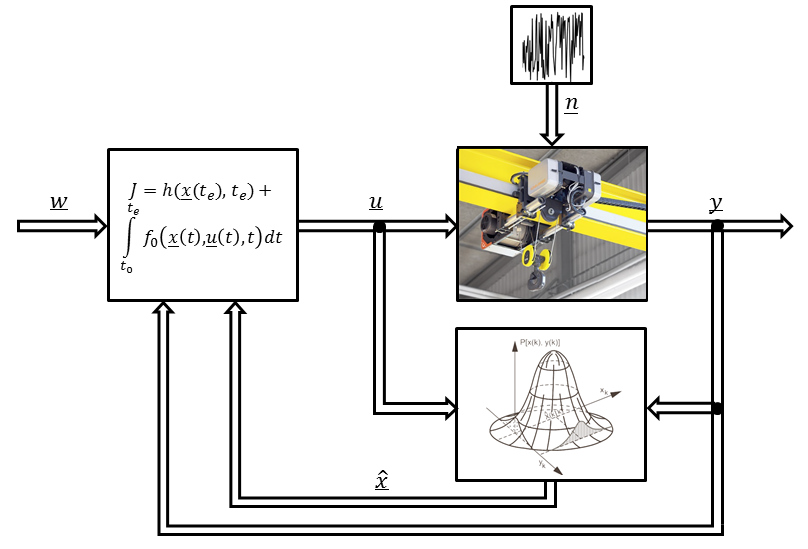
\includegraphics[width=\textwidth]{ors.png}}


\begin{document}
%------------------------Initialisierung------------------------%

% Definition for tikz package
\tikzstyle{vecArrow} = [thick, decoration={markings,mark=at position
1 with {\arrow[semithick]{open triangle 60}}},
double distance=1.4pt, shorten >= 5.5pt,
preaction = {decorate},
postaction = {draw,line width=1.4pt, white,shorten >= 4.5pt}]
\tikzstyle{dashArrow} = [dashed, decoration={markings,mark=at position
1 with {\arrow[semithick]{open triangle 60}}},
double distance=1.4pt, shorten >= 5.5pt,
preaction = {decorate},
postaction = {draw,line width=1.4pt, white,shorten >= 4.5pt}]  
\tikzstyle{innerWhite} = [semithick, white,line width=1.4pt, shorten >= 4.5pt]

\tikzset{
block/.style    = {draw, thick, rectangle, minimum height = 2em,
minimum width = 2em},
bblock/.style    = {draw, thick, rectangle, minimum height = 4em,
minimum width = 2em},
sum/.style      = {draw, circle, node distance = 2cm}, % Adder
input/.style    = {coordinate}, % Input
output/.style   = {coordinate} % Output
}

\newcommand\encircle[1]{%
\tikz[baseline=(X.base)] \node (X) [draw, shape=circle, inner sep=0] {\strut #1};}

%-----------------------keiner Hauptteil------------------------%
\pagestyle{plain}
\maketitle
%---------------------------Vorwort-----------------------------%
\tableofcontents
\setcounter{page}{1}
\frontmatter
\addcontentsline{toc}{chapter}{Vorwort}
\chapter*{Vorwort}   
Dieses Skript geh"ort zur Vorlesung „Optimale Regelung und Sch"atzung“ vom Herrn Dr. Mathias Kluwe am Karlsruher Institut für Technologie (KIT), die ich im Sommersemester 2017 gehalten habe. Inhaltlich habe ich mich dabei an die Abschrift von Ruochen Wang und Xiaoyu Xie gehalten. \\[5pt]
Da die Vorlesung erstmal im Sommersemester 2016 gegeben ist, wurde dieses Skript erstmals zusammengestell. Es ist nicht
ausgeschlossen, dass sich trotz sorgf"altiger Durchsicht noch Fehler verbergen. Wer Lust hat ein wenig Korrektur zu lesen, oder wer Fehler, besonders inhaltlicher Art im Skript entdeckt, teile es mir bitte mit: {\color{blue}\href{mailto:jun.lou.chn@outlook.com}{jun.lou.chn@outlook.com}}\\[5pt]
Das Skript ist nur für den persönlichen Gebrauch der Studierenden der Mechatrinik/ Elektrotechnik und Informationstechnik am KIT vorgesehen und darf nicht in irgendeiner Art und Weise vervielfältigt oder ver"offentlicht werden. \\[5pt]
Für Kritik und Anregungen bin ich jederzeit dankbar.\\[6pt]
\begin{flushright} Jun Lou, am 12. September 2017\\
in Karlsruhe\end{flushright}
\setcounter{page}{1}
\mainmatter

\setcounter{chapter}{-1}
%--------------------------Kapitel 0----------------------------%
\chapter[Einleitung und "Ubersicht]{Einleitung und "Ubersicht}
Vorlesungsfokus: Ans"atze zum \uline{Entwurf optimaler Regelungen und Sch"atzeinrichtungen}, dabei wesentliche Randbedingungen:
\begin{itemize}
\item \uline{Streckenmodellierung} \begin{itemize}
\item Frequenzbereich (MIMO/ SISO- "Ubertragungsfunktion)
\item Zeitbereich (Zustandsraum) \begin{itemize}
\item linear / nichtlinear
\item zeitkontinuierlich / zeitdiskret
\item deterministisch / stochastisch
\end{itemize}
\end{itemize}
\item \uline{Optimalit"atsanforderung} \begin{itemize}
\item G"utema"se
\item Optimierungsmethode
\end{itemize}
\end{itemize}
\clearpage
%--------------------------Kapitel 1----------------------------%
%-------------------------Sektion 1.1---------------------------%
\chapter{Synthese optimaler Regelungen mittels LQ-Optimierung}
\section{Optimalsteuerung dynamischer Systeme mittels Hamilton-Verfahrens}
\begin{itemize}
    \item \uline{Systemmodell} (auch als Nebenbedingung - \uline{NB} bezeichnet):\\
    MIMO-System: im Allgemeinen nichtlineare Zeitbereichsdarstellung\\
    $\dot{\uline{x}}=\uline{f}(\mathop{\uline{x}}\limits_{(n,1)},\mathop{\uline{u}}\limits_{(p,1)},t)$
    \item \uline{Optimierungsg"utema"s:}\\
    $\underbrace{J}_{Bolzasche-}=\underbrace{h(\uline{x}(t_e),t_e)}_{Meyer-}+\underbrace{\int_{t_0}^{t_e} f_0 (\uline{x},\uline{u},t) dt}_{Lagrangeg"utema"s}$
    \item \uline{Randbedingungen} (RB):\\
    meistens $t_0$, $t_e$ gegeben mit\begin{itemize}
        \item $\uline{x}(t_0)=\uline{x}_0$ fest
        \item $\uline{z}(\uline{x}(t_e),t_e)=\uline{0}$: \quad  \uline{Zielmannigfaltigkeit}
    \end{itemize}
    \item \uline{Optimierungsmethode: Hamilton-Verfahren}\\
    dabei NB und RB werden mit sogenannter \uline{Lagrange-Multiplikatoren} $\mathop{\uline{\psi}(t)}\limits_{(n,1)}$ (f"ur NB) und $\mathop{\uline{\mu}(t)}\limits_{(q,1)}$ (f"ur RB) in das G"utema"s integriert\\
    $\displaystyle J=h-\underbrace{\uline{\mu}^T\uline{z}}_{=\uline{0}}+\int_{t_0}^{t_e}\underbrace{(f_0-\uline{\psi}^T[\underbrace{\uline{f}-\dot{\uline{x}}}_{=\uline{0}}])}_{-H(\uline{x},\uline{\psi},\uline{u},t)\text{ \uline{Hamilton-Fkt}}}dt=J(\uline{x},\uline{\psi},\uline{u},t)\quad\text{   \uline{Funktional!}}$\\
    \uline{L"osungsprinzip: Variationsansatz}, um das Optimum mit klassischer Extremwertrechnung bestimmen zu k"onnen\\
    \fbox{$\uline{x}=\uline{x}^*+\lambda\uline{\eta}(t)$} \quad $x^*$, $u^*$ optimale Gr"o"sen, fest\\
    \fbox{$\uline{u}=\uline{u}^*+\lambda\uline{\xi}(t)$} \quad $\underbrace{\uline{\eta}(t),\quad\uline{\xi}(t)}_{\text{1. Varaition um }x^*,u^*}$ beliebig, fest\\
    damit: $J(\uline{x},\uline{\psi},\uline{u},t)\stackrel{!}{=}J(\lambda)$ $\Rightarrow$ einzig freier Parameter\\ $\Rightarrow$ Optimierung mittels Extremwertrechnung m"oglich\\
    $\uline{x}^*$, $\uline{u}^*$ aus \fbox{$\frac{dJ}{d\lambda} \Big |_{\lambda=0}=0$}
    \item \uline{Resultat} (ohne Herleitung): \\\uline{notwendige Bedingungen f"ur das Hamilton-Verfahren} \fbox{s. BB. ORS 1-1, 1-2}
\end{itemize}
%-------------------------Sektion 1.2---------------------------%
\section{Optimale Regelung linearer Prozesse mit quadratischem G"utekriterium}
\begin{itemize}
    \item \uline{Systemmodell:} MIMO, linear, kein Durchgriff\\
    $\uline{\dot{x}}=\uline{Ax}+\uline{Bu}$, \quad $\uline{x}(t_0)=\uline{x}_0$\\
    \uline{Annahmen:} \begin{itemize}
        \item $\uline{A}$, $\uline{B}$ $\uline{C}$ auch zeitvariant zul"assig
        \item $\uline{u}$, $\uline{x}$ unbeschr"ankt
    \end{itemize}
    \item \uline{G"utema"s} (enth"alt \uline{quadratische Formen}):\\
    $\displaystyle J=\frac{1}{2}\uline{x}^T(t_e)\uline{Sx}(t_e)+\frac{1}{2}\int_{t_0}^{t_e}[\uline{x}^T(t)\uline{Qx}(t)+\uline{u}^T(t)\uline{Ru}(t)]dt$ \quad mit \begin{itemize}
    \item $\uline{S}$, $\uline{Q}$ konstant, symmetrisch, positiv semidefinit ($\ge \uline{0}$)
    \item $\uline{R}$ konstant, symmetrisch, positiv definit (>$\uline{0}$)
\end{itemize}
\quad \quad ($\uline{Q}$, $\uline{R}$ auch zeitvariant zul"assig)\\
\uline{Ziel:} Optimalregelung $\uline{u}^*=\uline{u}^*(\uline{x},t)$, die das System stabilisiert, d.h. $\uline{x}(t_e)$ nach $\uline{0}$ "uberf"uhrt\\
\uline{Problem:} Idealforderung $\uline{x}(t_e)=\uline{0}$ liefert zu hohen Amplituden von $\uline{u}$ \\
$\Rightarrow$ $\uline{x}(t_e)\rightarrow\uline{0}$ durch hohes Gewicht von $\uline{S}$!
    \item \uline{Randbedingungen:} $t_0$, $t_e$ gegeben mit \begin{itemize}
        \item $\uline{x}(t_0)=\uline{x}_0$ fest
        \item $\uline{x}(t_e)$ frei
    \end{itemize}
\end{itemize}
%-----------------------Subsektion 1.2.1-------------------------%
\subsection{Optimale Regelung bei endlichem Zeitintervall}
\begin{enumerate}
    \item \uline{Hamilton-Verfahren} \fbox{s. BB. ORS 1-1, 1-2}\\[2pt]
    \uline{Hamilton-Funktion:} $\displaystyle H=-f_0+\uline{\psi}^T\uline{f}=-\frac{1}{2}\uline{x}^T\uline{Qx}-\frac{1}{2}\uline{u}^T\uline{Ru}+\uline{\psi}^T(\uline{Ax}+\uline{Bu})$
    \item \uline{Optimalsteuerung}\\[2pt]
    $\displaystyle\frac{\partial H}{\partial \uline{u}}\Big|_*=-\uline{Ru}^*+\uline{B}^T\uline{\psi}^*\stackrel{!}{=}\uline{0}$ $\Rightarrow$ \fbox{$\uline{u}^*=\uline{R}^{-1}\uline{B}^T\uline{\psi}^*$} ($\uline{R}^{-1}>\uline{0}$ f"ur $\uline{R}>\uline{0}$)
    \item \uline{Optimalregelung}\\[2pt]
    $\displaystyle \uline{\dot{x}}^*=\frac{\partial H}{\partial \uline{\psi}}\bigg|_*=\uline{Ax}^*+\uline{Bu}^*=\uline{Ax}^*+\uline{BR}^{-1}\uline{B}^T\uline{\psi}^*$ \quad (1)\\
    $\displaystyle\uline{\dot{\psi}}^*=-\frac{\partial H}{\partial \uline{x}}\Big|_*=\uline{Qx}^*-\uline{A}^T\uline{\psi}^*$ \quad (2)
    \item \uline{Randbedingungen:} 
    \begin{itemize}
        \item $\uline{x}(t_0)=\uline{x}_0$
        \item $\uline{x}(t_e)$ frei.\quad $\displaystyle\uline{\psi}^*(t_e)=-\frac{\partial h}{\partial \uline{x}}\bigg|_{t_e^*}=-\uline{Sx}^*(t_e)$ \quad (3)\\
    \end{itemize}
    (3) sowie die gew"unschte Reglerstruktur $\uline{u}=-\uline{Kx}$ motiviert den \uline{allgemeinen L"osungsansatz} \fbox{$\uline{\psi}^*=-\mathop{{\uline{P}(t)}}\limits_{(n,n)}\uline{x}^*$} \quad (4) \\
    \begin{center} 
    (4) in (2):\quad  $\uline{\dot{\psi}}^*={(-\uline{Px}^*)}^\cdot=-\uline{\dot{P}x}^*-\uline{P\dot{x}}^*\mathop{=}\limits_{(2)}^!=\uline{Qx}^*+\uline{A}^T\uline{Px}^* $\\
    $\Downarrow \uline{\dot{x}}^* \text{aus (1)}$\\
    $-\uline{\dot{P}x}^*-\uline{P}(\uline{Ax}^*-\uline{BR}^{-1}\uline{B}^T\uline{Px}^*)=\uline{Qx}^*+\uline{A}^T\uline{Px}^*$\\
    $\text{bzw. } (\uline{\dot{P}}+\uline{PA}-\uline{PBR}^{-1}\uline{B}^T\uline{P}+\uline{Q}+\uline{A}^T\uline{P})\uline{x}^*=\uline{0}$\\
    $\Downarrow \uline{x}^* \text{ beliebig}$\\        
    \fbox{$\dot{\uline{P}}(t)=-\uline{P}(t)\uline{A}-\uline{A}^T\uline{P}(t)+\uline{P}(t)\uline{BR}^{-1}\uline{B}^T\uline{P}(t)-\uline{Q}$}  \quad (5)  \uline{Matrix-Riccati-Dgl.}
    \end{center}
    Eigenschaften von $\uline{P}$ (ohne Beweis):\begin{itemize}
        \item $\uline{P}$ symmetrisch ($\Rightarrow \frac{n(n+1)}{2}$ verdoppelte Dgln. l"osen)
        \item $\uline{P}\ge \uline{0}$ (positiv semidefinit)
    \end{itemize}
    Vergleich von (3) und (4): Zur L"osung von (5) liegt eine Endbedingung von $\uline{P}(t_e)=\uline{S}$ vor $\Rightarrow$ durch Substitution \fbox{$\tau:=t_e-t$}\\
    "Uberf"uhrung von (5) mit \fbox{$\displaystyle\frac{d\uline{P}}{d\tau}=\uline{P}\uline{A}+\uline{A}^T\uline{P}-\uline{P}\uline{BR}^{-1}\uline{B}^T\uline{P}+\uline{Q}$} in ein „normales“ Anfangswertproblem $\uline{P}(\tau=0)=\uline{S}$ (vgl. ODS-Vorlesung)\\
    $\Rightarrow$ L"osung meist vorab (offline) unter Abspeicherung des Verlaufs von $\uline{P}(t)$\\
    mit L"osung von (5) sowie (4) und (2):\\
    $\uline{u}^*=-\underbrace{\uline{R}^{-1}\uline{B}^T\uline{P}(t)}_{=:\uline{K}(t)}\uline{x}^*$: \quad \fbox{$\uline{u}(\uline{x},t)=-\uline{K}(t)\uline{x}(t)$} \quad \uline{optimale zeitvariante Regelung}\\
    \uline{Beispiel}: \fbox{s. BB. ORS 1-3, 1-4}
\end{enumerate}
%-----------------------Subsektion 1.2.2-------------------------%
\subsection{Optimale Regelung bei unendlichem Zeitintervall}
aus 1.2.1 motiviert (vgl. \fbox{BB. ORS 1-4})\\
\uline{Ansatz} $t_e \rightarrow \infty$, um einen zeitinvarianten Regler ($\uline{K}(t)=\uline{K}!$) zu erhalten\\
$\Rightarrow$ Modifikation der Voraussetzungen erforderlich
\begin{itemize}
    \item \uline{Systemmodell}: \quad $\dot{\uline{x}}=\uline{Ax}+\uline{Bu}, \quad \uline{x}(t_0)=\uline{x}_0$ mit $\uline{A}, \uline{B}$ konst.\\
    \begin{tabular}{ll}
        \uline{Voraussetzung}: & a) System steuerbar  (Zust"ande beeinflussbar)\\
            & b) System beobachtbar bei $\uline{y}=\uline{Cx}$ \quad mit $\uline{C}^T\uline{C}=\uline{Q}(s)$
    \end{tabular}
    \item \uline{G"utema"s}: \quad  $\displaystyle J=\frac{1}{2}\int_{t_0}^{\infty}[\uline{x}^T\uline{Qx}+\uline{u}^T\uline{Ru}]dt$ \quad mit \begin{itemize}
        \item $\uline{Q}$ konstant, symmetrisch, positiv semidefinit ($\ge \uline{0}$)
        \item $\uline{R}$ konstant, symmetrisch, positiv definit($>\uline{0}$)
    \end{itemize}
\end{itemize}
\uline{Anmerkungen}: \begin{itemize}
    \item Zeitinvarianz erfordert $\uline{A}, \uline{B}$ konstant
    \item Voraussetzung a) und b) stelle sicher, dass $\mathop{\text{lim}}\limits_{t_e\rightarrow \infty} \uline{x}(t)=\uline{0}$ gilt und jeder Zustand im G"utema"s sichtbar bleibt. (\uline{Alternative}: $\uline{Q}$ positiv definit ($>\uline{0}$) )
    \item Meyesches G"utema"s entf"allt wegen $\mathop{\text{lim}}\limits_{t_e\rightarrow \infty}\uline{x}(t)=\uline{0}$, analoge Herleitung wie im 1.2.1:\\
    $\uline{P}(t)=\uline{P}_0=\text{konst.}$ bei R"uckwertsintegration, da auch f"ur $\uline{P}_0$ Riccati-Dgl. (s. 1.2.1) g"ultig mit $\uline{P}_0=\uline{0}$\\
    \fbox{$\uline{P}_0\uline{A}+\uline{A}^T\uline{P}_0-\uline{P}_0\uline{BR}^{-1}\uline{B}^T\uline{P}_0+\uline{Q}=\uline{0}$} \quad \uline{algebraische Matrix-Riccati-Dgl.} \\(station"are Matrix-Riccati Dgl.)\\ (eindeutig l"osbar f"ur Vorausssetzung a) !)\\
    $\Rightarrow$ \fbox{$\uline{u}=-\underbrace{\uline{R}^{-1}\uline{B}^T\uline{P}_0}_{=:\uline{K}}\uline{x}$} \quad \uline{zeitinvariantes Regelungsgesetz Riccati-Regler}\\
    \uline{Beispiel}: \uline{Verladebr"ucke} \fbox{s. BB. ORS 1-5 bis 1-8}    
\end{itemize}
%-----------------------Subsektion 1.2.3-------------------------%
\subsection{Optimale Regelung mit St"orgr"o"senunterdr"uckung}
\begin{tabular}{ll}
    \uline{bisher}:& nur Anfangsst"orungen $\uline{x}(t_0)$ betrachtet \\
    \uline{jetzt}: & bekannte St"orgr"o"sen $\uline{z}(t)$ zugelassen
\end{tabular}
\begin{itemize}
    \item \uline{Systemmodell} (Nebenbedingungen): \quad $\uline{\dot{x}}=\underbrace{\uline{Ax}+\uline{Bu}+\uline{z}}_{\uline{f}(\uline{x},\uline{u},\uline{z},t)}$ \quad $\mathop{z(t)}\limits_{(n,1)}$ messbar in $[t_0, t_e]$
    \item \uline{G"utema"s}: \quad $\displaystyle J=\frac{1}{2}\uline{x}^T(t_e)\uline{Sx}(t_e)+\frac{1}{2}\int^{t_e}_{t_0}\underbrace{[\uline{x}^T\uline{Qx}+\uline{u}^T\uline{Ru}]}_{=2\cdot f_0(\uline{x},\uline{u},t)}dt$
\end{itemize}
\uline{Hamilton-Verfahren} (vgl. \fbox{BB. ORS 1-1} bzw. 1.2.1) \begin{enumerate}
    \item \uline{Halmilton-Funktion}:\quad $H=-f_0+\uline{\psi}^T\uline{f}=-\frac{1}{2}(\uline{x}^T\uline{Qx}+\uline{u}^T\uline{Ru})+\uline{\psi^T}(\uline{Ax}+\uline{Bu}+\uline{z})$
    \item \uline{Optimalsteuerung}:\quad $\displaystyle\frac{\partial H}{\partial \uline{u}}\bigg|_*=-\uline{Ru}^*+\uline{B}^T\uline{\psi}^*\stackrel{!}{=}\uline{0}$ $\Rightarrow$ \fbox{$\uline{u}^*=\uline{R}^{-1}\uline{B}^T\uline{\psi}^*$} \quad (1)
    \item \uline{Optimalregelung}:\\[3pt]
    $\displaystyle\uline{\dot{x}}^*=\frac{\partial H}{\partial \uline{\psi}}\bigg|_*=\uline{Ax}^*+\uline{Bu}^*+\uline{z}$ \quad (2)\\
    $\displaystyle\uline{\dot{\psi}}^*=-\frac{\partial H}{\partial \uline{x}}\bigg|_*=\uline{Qx}^*-\uline{A}^T\uline{\psi}^*$ \quad (3)
\end{enumerate}
Transversalit"atsbedingung (s. fr"uher): \quad $\uline{x}(t_e)$ frei: \quad \fbox{$\uline{\psi}^*(t_e)=-\uline{Sx}^*(t_e)$}\\
analog zu 1.2.1 L"osungsansatz
\center \fbox{$\uline{\psi}^*(t)=-\uline{P}(t)\uline{x}^*(t)-\underbrace{\uline{p}(t)}_{(n,1)}$} \quad (4) \quad Ber"ucksichtigung der St"orung
\flushleft dabei:\quad $\uline{P}(t_e)=\uline{S}, \quad \uline{p}(t_e)=\uline{0}$\\
$\uline{\dot{\psi}}^*=-\uline{\dot{P}}\uline{x}^*-\uline{P\dot{x}}^*-\uline{\dot{p}}\mathop{=}\limits_{(3)}^{!}\uline{Qx}^*-\uline{A}^T\uline{\psi}^*\stackrel{(4)}{=}\uline{Qx}^*+\uline{A}^T\uline{Px}^*+\uline{A}^T\uline{p}$\\
also mit NB und (1):\\
$-\uline{\dot{P}x}^*-\uline{PAx}^*+\uline{PBR}^{-1}\uline{B}^T(\uline{Px}^*+\uline{p})-\uline{Pz}-\uline{\dot{p}}=\uline{Qx}^*+\uline{A}^T\uline{Px}^*+\uline{A}^T\uline{p}$\\
$\Rightarrow$ $\Big(\uline{\dot{P}}+\uline{PA}+\uline{A}^T\uline{P}-\uline{PBR}^{-1}\uline{B}^T\uline{P}+\uline{Q}\Big)\uline{x}^*+\uline{\dot{p}}+\Big(\uline{A}^T-\uline{PBR}^{-1}\uline{B}^T\Big)\uline{p}+\uline{Pz}=\uline{0}$ \quad (5)\\
da (5) f"ur $\uline{P}(t)$ und $\uline{p}(t)$ g"ultig ist, folgt\\
\fbox{$\uline{\dot{P}}(t)=-\uline{P}(t)\uline{A}-\uline{A}^T\uline{P}(t)+\uline{P}(t)\uline{BR}^{-1}\uline{B}^T\uline{P}(t)-\uline{Q}$} \quad (6)\\
Matrix-Riccati-Dgl.\quad (Endwertbedingung: $\uline{P}(t_e)=\uline{S}$)\\
\fbox{$\uline{\dot{p}}(t)=-(\uline{A}^T-\uline{P}(t)\uline{BR}^{-1}\uline{B}^T)\uline{p}(t)-\uline{P}(t)\uline{z}$} \quad (7)\\
"Vektor-Dgl."\quad (Endwertbedingung: $\uline{p}(t_e)=\uline{0}$)\\
wie 1.2.1 L"osung von (6) und (7) durch R"uckw"artsintegration\\
$\Rightarrow$ $\uline{P}(t)$ und $\uline{p}(t)$ in (1) ergibt $\uline{u}^*$ und $\uline{u}$\\
\fbox{$\uline{u}(\uline{x},\uline{p},t)=-\underbrace{\uline{R}^{-1}\uline{B}^T\uline{P}(t)\uline{x}(t)}_{\text{Zustandsr"uckf"uhrung}}-\underbrace{\uline{R}^{-1}\uline{B}^T\uline{p}(t)}_{\text{St"orgr"o"senaufschaltung}}=\underbrace{-\uline{K}_R\uline{x}}_{\uline{u}_R}\underbrace{-\uline{K}_z(z)}_{\uline{u}_z}$} \quad (8)\\
$\rightarrow$ \uline{Optimale Zeitvariable Regelung mit St"orgr"o"senunterdr"uckung}\clearpage
\uline{Struktur}:\\[6pt]
\begin{tikzpicture}[auto, node distance=2cm, >=triangle 45]
    \draw % set the nodes :
        node at (0,0)[block] (pt) {\large $p(t)$}
        node [sum, below of=pt] (suma) {}
        node [block, right of=suma] (RB) {\large $\uline{R}^{-1}\uline{B}^T$}
        node [block, right of=RB, right=1cm] (ZF) {\large $\uline{\dot{x}}=\uline{Ax}+\uline{Bu}+\uline{z}$}
        node [block, below of=RB] (Pt) {\Large$-\uline{P}(t)$}
        node at (6,-0.75) (x0) {\large $\uline{x}_0$}
        node at (8,-0.75) (zt) {\large $\uline{z}(t)$}
        node at (11,-2) (ZFz) {\large}
        node at (6,0) (sieben) {\large $(7)$}
        node at (-0.4,-1.6) {$-$};
    % link the nodes [vecArrow] and [->] 
    \draw[vecArrow](pt) -- (suma);
    \draw[vecArrow](suma) -- (RB);
    \draw[vecArrow](RB) -- node{$\uline{u}$}(ZF);
    \draw[vecArrow](Pt) -| (suma);
    \draw[vecArrow](x0) -- (6,-1.6);
    \draw[vecArrow](zt) -- (8,-1.6);
    \draw[vecArrow](ZF) --(11,-2) |- (Pt);
    \draw[vecArrow](sieben) -- (pt);
    \draw[vecArrow](sieben) -| (zt);
    \draw [dashed](-1,-5) rectangle (4.2,1);
    \node at (-0.5,-6) [above=5mm, right=0mm] {\text{optimaler LQ-Regler}};
\end{tikzpicture}\\
\uline{Anmerkungen}:
\begin{itemize}
    \item \uline{Spezialfall} \quad $\uline{z}=\uline{0}$ \quad (7): \quad $\uline{\dot{p}}+\Big(\uline{A}^T-\uline{PBR}^{-1}\uline{B}^T\Big)\uline{p}=\uline{0}$ mit $\uline{p}(t_e)=\uline{0}$\\
    $\Rightarrow$ $\uline{p}(t)=\uline{0}$ in [$t_0, t_e$] \quad \uline{Standard LQ-Problem}
    \item \uline{Spezialfall}\quad $\uline{z}=\uline{\overline{z}}=$konst. und $t_e\rightarrow\infty$\\
    $\Rightarrow$ Station"are L"osung f"ur die Dgln. (6), (7)\\
    $\uline{K}_R=\uline{R}^{-1}\uline{B}^T\uline{P}_0$ in (7) (s. 1.2.2)\\
    $\uline{p}(t)=\uline{p}_0=$konst. $\Rightarrow$ $\uline{\dot{p}}_0=\uline{0}$ $\Rightarrow$ $\uline{p}_0=-(\uline{A}^T-\uline{P}_0\uline{BR}^{-1}\uline{B}^T)^{-1}\uline{P}_0\uline{\overline{z}}$\\
    $\uline{u}_z=-\underbrace{\uline{R}^{-1}\uline{B}^T(\uline{A}^T-\uline{P}_0\uline{BR}^{-1}\uline{B}^T)^{-1}\uline{P}_0}_{=:\uline{K}_z}\uline{\overline{z}}$\\
    \uline{Struktur}:\\[6pt]
    \begin{tikzpicture}[auto, node distance=2cm, >=triangle 45]
        \draw % set the nodes :
            node at (0,0) [block] (KZ) {\large $\uline{K}_Z$}
            node [sum, below of=KZ] (suma) {}
            node [block, right of=suma, right=0cm] (ZF) {\large $\uline{\dot{x}}=\uline{Ax}+\uline{Bu}+\uline{z}$}
            node [block, below of=suma] (KR){\large $\uline{K}_R$}
            node at (3,-0.75) (x0) {\large $\uline{x}_0$}
            node at (3,0) (z) {\large $\uline{\overline{z}}$}
            node at (0.3,-2.3) {$-$}
            node at (-0.3,-1.7) {$-$};
        % link the nodes [vecArrow] and [->] 
        \draw[vecArrow](KZ) -- node{$\uline{u}_Z$}(suma);
        \draw[vecArrow](KR) -- node{$\uline{u}^*$}(suma);
        \draw[vecArrow](suma) -- node{$\uline{u}$}(ZF);
        \draw[vecArrow](ZF) -- node{$\uline{x}$}(8,-2);
        \draw[vecArrow](7,-2) |- (KR);    
        \draw[innerWhite](6.5,-2) |- (7.5,-2);
        \draw[vecArrow](z) -- (KZ);
        \draw[vecArrow](z) -- (4.5,0) -- (4.5,-1.6);
        \draw[vecArrow](x0) -- (3,-1.6);
        \draw[dashed](-1,-5) rectangle (0.8,1);
        \node at (-0.5,-6) [above=5mm, right=0mm] {LQ-Regler mit station"arer St"orgr"o"senaufschaltung};
    \end{tikzpicture}\\
    (\uline{Achtung}: $\uline{x}(t_e\rightarrow\infty)\neq\uline{0}$ ist m"oglich, da Optimalregler den St"oreinfluss auf $\uline{u}$ und $\uline{x}$ verteilt!)
    \item bei nicht messbarer St"orung: \uline{Ansatz mit St"ormodell}, dazu \uline{St"ormodell $\uline{\dot{z}}=\uline{Fz}$ sei bekannt}\\
    dann f"ur erweiterten Modell\\[2pt]
    $\begin{bmatrix} \uline{x}\\\uline{z}\end{bmatrix}^{\cdot} = 
    \begin{bmatrix} \uline{A} & \uline{I}\\\uline{0} & \uline{F}\end{bmatrix} \begin{bmatrix} \uline{x}\\ \uline{z} \end{bmatrix}+ \begin{bmatrix} \uline{B}\\ \uline{0} \end{bmatrix}\uline{u}$\\[2pt]
    Entwurf einer LQ-Regelung wie in 1.2.1 $\Rightarrow$ $\uline{u}(t)=-\uline{K}_x\uline{x}-\uline{K}_z\uline{z}$
\end{itemize}
\clearpage
%-----------------------Subsektion 1.2.4-------------------------%
\subsection{Optimale Folgeregelung}
\begin{tabular}{ll}
    \uline{bisher}:& verschwindende Sollwerte f"ur $\uline{x}$, $\uline{u}$\\
    \uline{jetzt}: & Vorgabe \uline{gew"unschter Sollwertverl"aufe $\uline{x}_s(t)$, $\uline{u}_s(t)$}\\
    & $\rightarrow$ \uline{optimale Folgeregelung} \quad (Dynamik $\uline{\dot{x}}_s=\uline{A}_s\uline{x}_s+\uline{B}_s\uline{u}_s$)
\end{tabular}\\
\uline{Definition}: \uline{Abweichungen} $\Delta\uline{x}:=\uline{x}-\uline{x}_s$, $\Delta\uline{u}:=\uline{u}-\uline{u}_s$
\begin{itemize}
    \item \uline{G"utema"s}: \quad
    $\displaystyle J=\frac{1}{2}\Delta\uline{x}^T(t_e)\uline{S}\Delta\uline{x}(t_e)+\frac{1}{2}\int^{t_e}_{t_0}[\Delta\uline{x}^T\uline{Q}\Delta\uline{x}+\Delta\uline{u}^T\uline{R}\Delta\uline{u}]dt$ \\
    \begin{tabular}{ll}
        mit& - $\uline{S}, \uline{Q}\geq\uline{0}$ und $\uline{R}>\uline{0}$\\
        & - $\uline{Q}, \uline{R}$ auch zeitvariant
    \end{tabular}
    \item \uline{Systemmodell(NB)}: \quad f"ur Abweichungen erfordlich $\Delta\uline{\dot{x}}=\uline{\dot{x}}-\uline{\dot{x}}_s=\uline{Ax}+\uline{Bu}-\uline{\dot{x}}_s\stackrel{!}{=}\uline{A}\Delta\uline{x}+\uline{B}\Delta\uline{u}+\underbrace{\uline{Ax}_s+\uline{Bu}_s-\uline{\dot{x}}_s}_{=:\uline{z}}$ \quad (1)\\
    \uline{also} R"uckf"uhrung auf St"orgr"o"senunterdr"uckung m"oglich!\\
    \uline{Fallunterscheidung} f"ur (1), \uline{Sollwertverl"aufe} 
    \begin{itemize}
        \item \uline{gehorchen der Systemdynamik der Strecke}\\
        $\uline{A}_s=\uline{A}$, $\uline{B}_s=\uline{B}$, d.h. $\uline{\dot{x}}_s=\uline{Ax}_s+\uline{Bu}_s$\\
        $\Rightarrow$ $\uline{z}=\uline{0}$: Standard-LQ-Optimierung (vgl. 1.2.1) f"ur $\Delta\uline{x}$, $\Delta\uline{u}$\\
        $\Rightarrow$ $\Delta\uline{u}=-\uline{R}^{-1}\uline{B}^T\uline{P}\Delta\uline{x}$ bzw. \fbox{$\uline{u}=-\uline{R}^{-1}\uline{B}^T\uline{Px}+\uline{R}^{-1}\uline{B}^T\uline{Px}_s+\uline{u}_s$}
        \item \uline{gehorchen nicht der Systemdynamik der Strecke}\\
        $\uline{z}\neq\uline{0}$ aber bekannt\\
        $\Rightarrow$ LQ-Optimierung mit St"orgr"o"senunterdr"uckung (vgl. 1.2.3) f"ur $\Delta\uline{x}$, $\Delta\uline{u}$\\
        $\Rightarrow$ $\Delta\uline{u}=-\uline{R}^{-1}\uline{B}^T\uline{P}\Delta\uline{x}-\uline{R}^{-1}\uline{B}^T\uline{p}(t)$ \quad bzw. \fbox{$\uline{u}=-\uline{R}^{-1}\uline{B}^T\uline{P}\uline{x}+\uline{R}^{-1}\uline{B}^T\uline{P}\uline{x}_s-\uline{R}^{-1}\uline{B}^T\uline{p}(t)+\uline{u}_s$}\\
        (dabei jeweils Dgln. f"ur $\uline{P}$ und $\uline{p}$ zu l"osen!)
    \end{itemize}
\end{itemize}
\uline{Struktur}:\\[6pt]
\begin{tikzpicture}[auto, node distance=2cm, >=triangle 45]
    \draw % set the nodes :
        node at (0,0) [block] (pt) {\large $\uline{p}(t)$}
        node [sum, below of=pt] (suma1) {}
        node [block, right of=suma1] (RB) {\large $\uline{R}^{-1}\uline{B}^T$}
        node [sum, right of=RB] (suma2) {}
        node [block, right of=suma2, right=0cm] (ZF) {\large $\uline{\dot{x}}=\uline{Ax}+\uline{Bu}$}
        node [block, below of=suma2] (P2){\large $\uline{P}$}
        node at (-0.3,-1.7) (){-}
        node at (0.3,-2.3) (){-}
        node at (6.5,-0.75) (x0) {\large $\uline{x}_0$}
        node at (4,0) (us) {\large $\uline{u}_s$}
        node [block, left of =suma1] (P1) {\large $\uline{P}$};
    % link the nodes [vecArrow] and [->] 
    \draw[vecArrow](pt) -- (suma1);
    \draw[vecArrow](P1) -- (suma1);
    \draw[dashArrow](-2.8,-2) |- (pt); 
    \draw[vecArrow](-4,-2) -- node{$\uline{x}_s$}(P1);
    \draw[vecArrow](P2) -| (suma1);
    \draw[vecArrow](suma1) -- (RB);
    \draw[vecArrow](RB) -- (suma2);
    \draw[vecArrow](suma2) -- node{$\uline{u}$}(ZF);
    \draw[vecArrow](ZF) -- node{$\uline{x}$}(10,-2) |-(P2);
    \draw[dashArrow](us) -- (pt);
    \draw[vecArrow](us) -- (suma2);
    \draw[vecArrow](x0) -- (6.5,-1.6);
    \draw[dashed](-4.5,-5) rectangle (4.8,1);
    \node at (-1.5,-6) [above=5mm, right=0mm] {Optimaler Folgeregler};
\end{tikzpicture}\\
\uline{Anmerkung}: falls nur $\uline{x}_s$ relevant: Wahl von $\uline{u}_s$ so, dass eine Systemtrajektorie durchlaufen wird ($\uline{p}=\uline{0}$) (= \uline{Vorsteuerung})
%-----------------------Subsektion 1.2.5-------------------------%
\subsection{Optimierung bei beschr"ankter Stellgr"o"sen: Das Maximumprizip von Pontrjagin}
\uline{bisher}: bei Hmilton-Verfahren $\frac{\partial H}{\partial\uline{u}}=\uline{0}$ (Steuerungsgleichung) (1) gefordert, wobei auch zeigen l"asst (ohne Herleitung):\\
\[\frac{\partial^2 H}{\partial\uline{u}^2}\leq\uline{0}, \quad \forall t\in [t_0, t_e] \]
d.h. (1) ist notwendige Bedingung f"ur ein \uline{Maximum von H}.\\
\fbox{$H(\uline{x}^*,\uline{\psi}^*,\uline{u}^*,t)\stackrel{!}{=}\mathop{max}\limits_{\uline{u}}$} \quad (2)\\
$\Rightarrow$ \uline{Problem}: (1) braucht bei \uline{beschr"ankten Stellgr"o"sen} (z.B. $\uline{m}\leq\uline{u}\leq\uline{M}$) nicht erf"ullt zu sein.\\
\uline{Beispiel}: \uline{Randmaximum}\\[6pt]
\begin{tikzpicture}
    \draw[-triangle 45] (-0.5,0) -- (5,0);
    \draw[-triangle 45] (0,-0.5) -- (0,4);
    \draw node at (0.5,4) {$H$};
    \draw node at (5,0.5) {$u$};
    \draw node at (3.5,2.5) {\Large $\frac{\partial H}{\partial u}\leq0$};
    \draw node at (0.5,-0.4) {$m$};
    \draw node at (4.2,-0.4) {$M$};
    \draw[dashed] (0.5,-0.1) -- (0.5,3.2);
    \draw[dashed] (4.2,-0.1) -- (4.2,0.3);
    \draw (0.3,3.3) -- (3,1.95);
    \draw [very thick](0.5,3.2) .. controls (1,2.8) and (2.8,2.3) .. (4.2,0.3);
\end{tikzpicture} \quad \quad 
\begin{tikzpicture}
    \draw[-triangle 45] (-0.5,0) -- (5,0);
    \draw[-triangle 45] (0,-0.5) -- (0,4);
    \draw node at (0.5,4) {$H$};
    \draw node at (5,0.5) {$u$};
    \draw node at (5.2,3.5) {\Large $\frac{\partial H}{\partial u}\geq0$};
    \draw node at (0.5,-0.4) {$m$};
    \draw node at (4.2,-0.4) {$M$};
    \draw[dashed] (0.5,-0.1) -- (0.5,1);
    \draw[dashed] (4.2,-0.1) -- (4.2,3.5);
    \draw (2.4,0.5) -- (4.4,3.83);
    \draw [very thick](0.5,1) .. controls (2.2,0.1) and (3,1.8) .. (4.2,3.5);
\end{tikzpicture}\\
\uline{Abhilfe}: Forderung (2) anstelle von (1) im Hamilton-Verfahren benutzen\\
$\Rightarrow$ \uline{Maximumprinzip im Pontrjagin} (1956) z.B. \fbox{s. BB. ORS 1-11, 1-12}\\
typische Anwendungsfall: zeitoptimale Regelung

%-----------------------aboved checked-------------------------%  

%-----------------------Subsektion 1.2.6-------------------------%
\subsection{Zeitoptimale Regelung}
Ziel: m"oglichst schnelle "Uberf"uhrung des Anfangszustands in den Endzustand, dabei\begin{itemize}
    \item \uline{Prozessmodell} (NB): \quad $\uline{\dot{x}}=\uline{Ax}+\uline{Bu}$, $\uline{x}(t_0)=\uline{x}_0$, $\uline{x}(t_e)=\uline{0}$ (fester Endpunkt)
    \item \uline{G"utem"a"s} \quad $J=\int_0^{t_e}1dt=t_e$ (also $t_0=0$, $t_e$ frei $\rightarrow$ Min)
    \item \uline{Besch"ankung der Stellgr"o"sen} \quad $\forall$ t \fbox{$m_k\leq u_k\leq\ M_k$} (k=1,...,p)
\end{itemize}
\uline{L"osung mittels Hamilton-Verfahren}\begin{enumerate}
    \item \uline{Hamilton-Funktion}: \quad $H=-f_0+\uline{\psi}^T\uline{f}=-1+\uline{\psi}^T\uline{Ax}+\underbrace{\uline{\psi}^T\uline{Bu}}_{=:\tilde{H}}$
    \item \uline{Optimale Steuergr"o"sen}: Maximumprinzip: optimales $\uline{u}^*$ f"ur $H=H_{max}$\\
    wegen 1.: $H_{max}$ liegt vor, wenn $\tilde{H}$ maximal wird\\
    $\displaystyle\tilde{H}=\uline{\psi}^T\uline{Bu}\stackrel{!}{=}\uline{u}^T\uline{B}^T\uline{\psi}=\uline{u}^T\begin{bmatrix}\uline{b}_1^T\\ \vdots\\\uline{b}_p^T\end{bmatrix}\uline{\psi}=\uline{u}^T\begin{bmatrix}\uline{b}_1^T\uline{\psi}\\ \vdots\\\uline{b}_p^T\uline{\psi}\end{bmatrix}=\sum^{p}_{k=1}u_k\uline{b}_k^T\uline{\psi}$\\
    also: $\tilde{H}$ maximal, wenn jeder Summand m"oglichst gro"s ist, d.h.: 
    $\uline{b}_k^T\uline{\psi}\left \{%
    \begin{array}{ll}
        >0: & u_k \text{ m"oglichst gro"s}\\
        <0: & u_k \text{ m"oglichst klein}\\
    \end{array} \right.$\\
    $\Rightarrow$ zeitoptimale Steuerfunktion $u_k^*(t)$
    \fbox{$u_k^*(t)=\left \{%
    \begin{array}{ll}
    m_k, & \uline{b}_k^T\uline{\psi}^*<0\\
    M_k, & \uline{b}_k^T\uline{\psi}^*>0\\
    \end{array} \right.$} \quad (1)\\
    \uline{also}: Umschaltung bei Vorzeichnenwechsel der \uline{Schaltfunktion} $S_k(t)=\uline{b}_k^T\uline{\psi}^*(t)$
    \begin{tikzpicture}
        \draw[-triangle 45] (-0.5,0) -- (9,0);
        \draw[-triangle 45] (0,-1.3) -- (0,1.8);
        \draw node at (2.6,1.4) {$u_k^*(t)$};
        \draw node at (9.5,0) {$t$};
        \draw node at (-0.6,1.5) {$M_k$};
        \draw node at (-0.6,-1) {$m_k$};
        \draw node at (8.6,1) {$S_k(t)$};
        \draw[very thick] (0,1) cos (2,0) sin (3.5,-0.8) cos (6,0) sin (8,1);
        \draw[very thick] (-0.1,1.2) -- (2,1.2) -- (2,-1)--(6,-1)--(6,1.2)--(8,1.2);
        \draw[dashed] (-0.1,-1) -- (2,-1);
    \end{tikzpicture}\\
    \uline{Sonderfall}: $m_k=-M_k$ $\Rightarrow$ \fbox{$u_k^*=M_k\text{sgn} (\uline{b}_k^T\uline{\psi}^*(t))$} \quad (2)\\
    \uline{Fazit}: optimale Steuerfunktion st"uckweise konstant bei dem Minimum bzw. Maximum ("\uline{bang-bang-control}")\\
    \begin{tabular}{ll}
        (\uline{Anmerkung}:& in (1) bzw. (2) $\uline{b}_k^T\uline{\psi}^*\neq0$ au"ser in einzelnen Nullstellen gefordert\\
        & $\Updownarrow$ wegen $\uline{\psi}^*(t)\neq\uline{0}$ (BB. ORS 1-12) gilt (ohne Herleitung)\\
        & $\uline{Q}_k=[\uline{b}_k, \uline{Ab}_k, \cdots, \uline{A}^{n-1}\uline{b}_k]$ regul"ar, d.h.\\
        & Strecke muss um jedem $u_k$ vollst"andig steuerbar sein!)
    \end{tabular}
    \uline{Bestimmung von $\uline{\psi}^*(t)$ f"ur (1) bzw. (2)}\\
    $\uline{\dot{\psi}}^*(t)=-\frac{\partial H}{\partial\uline{x}} \bigg|_*=-\uline{A}^T\uline{\psi}^*$ (nicht von $\uline{x}^*$ abh"angig!) $\Rightarrow$ $\uline{\psi}^*(t)=e^{-\uline{A}t}\uline{\psi}^*(0)$\\
    Bestimmung von $\uline{\psi}^*(0)$ und $t_e$: aus Endebedingung $\uline{x}(t_e)=\uline{0}$\\
    Es gilt allgemein (z.B. RLM-Vorlesung):\\
    $\displaystyle\uline{x}(t)=e^{\uline{A}t}\uline{x}(0)+\int_0^te^{\uline{A}(t-\tau)}\uline{Bu}(\tau)d\tau$\\
    $\bigg\Downarrow \left.
    \begin{array}{ll}
    \cdot \quad \uline{Bu}=\sum_{k=1}^p\uline{b}_ku_k\\
    \cdot \quad \text{Endebedingung: } \uline{x}(t_e)=\uline{0}\\
    \end{array} \right.$\\
    $\displaystyle\uline{x}(t_e)=e^{\uline{A}t_e}[\uline{x}(0)+\int_0^te^{-\uline{A}\tau}\sum_{k=1}^p\uline{b}_ku_k(\tau)d\tau]\stackrel{!}{=}\uline{0}$\\
    $\Rightarrow$ z.B. (2)\\
    $\displaystyle\int_0^{t_e}e^{-\uline{A}\tau}\sum_{k=1}^p\uline{b}_kM_k\text{sgn}\bigg[\uline{b}_k^Te^{-\uline{A}\tau}\uline{\psi}^*(0)\bigg]d\tau=-\uline{x}(0)$ \quad (a)\\
    \uline{Problem}: nur n Gleichungen f"ur $\uline{\psi}^*(0)$ und $t_e$\\
    f"ur eine weitere Gleichung zusatzannahme an $\uline{\psi}^*(0)$ m"oglich\\
    $\displaystyle \sum_{k=1}^n\psi_k^{*^2}(0)=1$ \quad (b)\\
    (a) zusammen mit (b): n+1 Gleichungen f"ur $\uline{\psi}^*(0)$ und $t_e$ \\
    (nichtlinear, selten analytisch l"osbar)\\
    \uline{aber}: Wissen "uber genauen Verlauf von $\uline{\psi}^*(t)$ eigentlich nicht erfordlich, nur die Umschaltpunkte f"ur (1), (2) wichtig 
    \\$\Rightarrow$ \uline{Satz von Feldbaum}: \fbox{s.BB. ORS 1-13}\\
    damit Gleichung zur Berechnung der Schaltzeitpunkte zu erhalten\\
    \uline{Beispiel}: \fbox{s.BB. ORS 1-14 bis 1-17}    
\end{enumerate}
%-----------------------Subsektion 1.2.7-------------------------%
\subsection{Stabilit"atsreserve von Riccati-Reglern (SISO-Fall)}
\begin{tabular}{ll}
    \uline{bisher}:& Stabilit"at der LQ-Regelungen nicht explizit untersucht\\
    \uline{jetzt}: & Stabilit"atsverhaltensanalyse:\\
    & - Phasenreserve \\
    & - Amplitudenreserve
\end{tabular}\\
\uline{hierzu}: Zustandsr"uckf"uhrung als "klassische Regelungsstruktur" im Frequenzbereich interpretiert

\begin{tikzpicture}[auto, node distance=2cm, >=triangle 45]
    \draw % set the nodes :
        node at (0,0) [sum] (suma) {}
        node at (3,0) [block] (ZF) {\large $\uline{\dot{x}}=\uline{Ax}+\uline{Bu}$}
        node at (3,-1) [block] (k) {\large $\uline{k}$};
    % link the nodes [vecArrow] and [->] 
    \draw[vecArrow](ZF) --node{$\uline{x}$} (6,0) |- (k);
    \draw[vecArrow](k) -| (suma);
    \draw[vecArrow](suma)--node{$\uline{u}$} (ZF);
    \draw node at (6.5,-0.5) {$\Rightarrow$};
\end{tikzpicture}  
\begin{tikzpicture}[auto, node distance=2cm, >=triangle 45]
    \draw % set the nodes :
    node at (0,0) [sum] (suma) {}
    node at (3,0) [block] (ZF) {\large $(j\omega\uline{I}-\uline{A})^{-1}\uline{B}$}
    node at (6,0) [block] (k) {\large $\uline{k}$};
    % link the nodes [vecArrow] and [->] 
    \draw[vecArrow](ZF) --node{$\uline{x}$} (k);
    \draw[vecArrow](k) -- (7.5,0) -| (7.58,-1) -- (0,-1) -- (suma);
    \draw[vecArrow](suma)--node{$\uline{u}$} (ZF);
    \draw [dashed](1,-0.5) rectangle (6.8,0.5);
    \draw node at (4,-0.7) {$\uline{F}_0(j\omega)=\uline{k}(j\omega\uline{I}-\uline{A})^{-1}\uline{B}$ \quad (1)};
    \draw node at (4,-1.3){};
\end{tikzpicture}\\
(\uline{Annahme}: $\uline{k}$ sei als zeitinvarianter Riccati-Regler (vgl. 1.2.2) entworfen)\\
$\Rightarrow$ sogenannte \uline{Regeldifferentialgleichung} (Herleitung: \fbox{s. BB. ORS 1-18}) gilt:\\[3pt] $\uline{R}+\uline{B}^T(-j\omega\uline{I}-\uline{A})^{-1}\uline{Q}(j\omega\uline{I}-\uline{A})^{-1}\uline{B}=[\uline{I}+\uline{B}^T(-j\omega\uline{I}-\uline{A})^{-1}\uline{k}^T]\uline{R}[\uline{I}+\uline{k}(j\omega\uline{I}-\uline{A})^{-1}\uline{B}]$\\
\uline{SISO-Fall}:\\
$[1+\uline{b}^T(-j\omega\uline{I}-\uline{A}^T)^{-1}\uline{k}^T]r[1+\uline{k}(j\omega\uline{I}-\uline{A})^{-1}\uline{b}]=r\bigg|1+\uline{k}(j\omega\uline{I}-\uline{A})^{-1}\uline{b}\bigg|^2\stackrel{!}{\geq}r$\\
d.h. $\bigg|1+\uline{k}(j\omega\uline{I}-\uline{A})^{-1}\uline{b}\bigg|^2\geq 1$ bzw. $\bigg|1+F_0(j\omega)\bigg|^2\geq 1$ \quad (3)\\
Anschauliche Interpretation von (3) \fbox{s. BB. ORS 1-19, 1-20}\\
weiterhin ergibt sich f"ur etwaige \uline{Verst"arkungsvariationen} 
$F_0=\nu\uline{k}^T(j\omega\uline{I}-\uline{A})^{-1}\uline{b}$\\
$\rightarrow$ anstelle von -1 jetzt kritischer Punkt $-\frac{1}{\nu}$ betrachten\\
\begin{tikzpicture}
    \draw[-triangle 45] (0,0) -- (5.5,0);
    \draw[-triangle 45] (4,-2) -- (4,2);
    \draw[dashed] (2,0) circle (1.5);
    \draw (2,-0.1) -- (2,0.1);
    \draw (2.8,-0.1) -- (2.8,0.1);
    \draw node at (2,-0.3) {$-1$};
    \draw node at (2.8,-0.3) {$-\frac{1}{\nu}$};
    \draw (5,1.2) circle (0.2);
    \draw node at (5,1.2) {$z$};
\end{tikzpicture}\\
mit (3) gilt: $\mathop{-2<-\frac{1}{\nu}<0}\limits_{\Large{(\text{also } 2>\frac{1}{\nu}>0)}}$ bzw. $\mathop{\frac{1}{2}<\nu<+\infty}\limits_{\text{(ohne, instabil zu werden)}}$ \quad (4) \\
$\rightarrow$ Riccati-Regler hat unendlich hohe Amplitudenreserve!\\
\uline{Fazit}: Riccati-Regler besitzen gewisse Toleranz bzgl. Phasen- und Verst"arkungsvariation.

%--------------------------Kapitel 2----------------------------%
%-------------------------Sektion 2.1---------------------------%
\chapter{Synthese robuster Regelungen}
\section{Definition robuster Regelungen}
zumeist Basis des Reglerentwurfs: Systemmodell beim konkreten Einsatz\\
zwei F"alle unterscheidbar: \begin{enumerate}
    \item \uline{Modell und Realit"at stimmen "uberein} (Nominalfall)\\
    neben qualitativen (Stabilit"at) vor allem gew"unschte \uline{quantitative Eigenschaften} sichergestellt (z.B. gute F"uhrungs-/ St"orverhalten)
    \item \uline{Modell gibt Realit"at nur fehlerhaft wieder} (Realfall)\\
    zwei Fehlerarten:\begin{enumerate}
        \item \uline{Strukturierte Fehler}: Fehler, die sich struktuell abgrenzen lassen und eine Beschreibung erm"oglichen, z.B. \uline{Parameter"anderungen} im Prozess
        \item \uline{Unstrukturierte Fehler}: Fehler, die leichter modellierbar sind und meist dynamisch durch ihre Betr"age (Norm) abgesch"atzt werden.
    \end{enumerate}
\end{enumerate}
\uline{Robuster Regler}: Regler, der nicht nur die quatitativen Anforderungen im Nominalfall erf"ullt, sondern auch den Realfall beherrscht (in bestimmten Grenzen, so z.B. wenn die Prozessver"anderungen langsam gegen"uber Prozessdynamik)\\
Hier \uline{zwei Verfahren} behandelt:\begin{itemize}
    \item H${}_\infty$-Methodik (Frequenzbereich)
    \item Polbereichsvorgabe (Zeitbereich)
\end{itemize}
%-------------------------Sektion 2.2----------------------------%
%-----------------------Subsektion 2.2.1-------------------------%
\section{Synthese robuster Regelung mittels H${}_\infty$-Minimierung}
\subsection{Grundlagen, Normen und Singul"arwertzerlegung}
f"ur sp"ateren Entwurf wichtig: Absch"atzung vektorieller Gr"o"sen und Abbildung $\rightarrow$ \uline{Normen} \fbox{s. BB. ORS 2-1, 2-2}\\
"Ubertragung auf lineare Abbildung: \uline{Operatornorm}\\
SISO-Fall: $y=ax$ $\Rightarrow$ $|y|=|a||x|$ darin ist $a$ die Verst"arkung\\
MIMO-Fall: Verst"arkung richtungsabh"angig\\
Beispiel: $\uline{y}=\uline{Ax}$ mit $\uline{A}=\begin{bmatrix} 0&10\\1&0\\\end{bmatrix}$ \quad $\underbrace{\uline{x}_1=\begin{bmatrix}1\\0\end{bmatrix},\quad \uline{x}_2=\begin{bmatrix}0\\1\end{bmatrix}}_{||\uline{x}_1||_2=||\uline{x}_2||_2=1}$\\
$\Rightarrow$ $\uline{y}_1=\uline{Ax}_1=\begin{bmatrix}0\\1\end{bmatrix}, ||\uline{y}_1||_2=1$,\quad $\uline{y}_2=\uline{Ax}_2=\begin{bmatrix}10\\0\end{bmatrix}, ||\uline{y}_2||_2=10$\\
\uline{Definition} \uline{Operatornorm}: \\
Bei der linearen Abbildung $\uline{y}=\uline{Ax}$ gilt \fbox{$\displaystyle||\uline{A}||_p=\mathop{max}\limits_{||\uline{x}||_p\neq0}\frac{||\uline{y}||_p}{||\uline{x}||_p}$} (maximale Verst"arkung)
\begin{tabular}{ll}
    \uline{Anmerkungen}:& - \uline{induzierte Norm} (abh"angig von Normen der Ein-/Ausg"ange)\\
    & - \uline{Submultiplikativ} mit $\uline{z}=\uline{By}$ gilt f"ur $\uline{z}=\uline{BAx}$,\quad $||\uline{BA}||_p\leq||\uline{B}||_p||\uline{A}||_p$ 
\end{tabular}\\
konkrete Berechnung "uber die \uline{Singul"arwertzerlegung}(SVD) der Matrix: \fbox{s. BB. ORS 2-3, 2-4}\\

\begin{tabular}{ll}
    denn gilt f"ur Abbildung & $\uline{y}=\uline{Ax}$\\
    & $\uline{A}=\uline{U\Sigma V}^*$\\
    & $\Downarrow$ $\uline{V}$ unit"ar     $\uline{V}^*\uline{V}=\uline{I}$\\
    & $\uline{AV}=\uline{U\Sigma}$ bzw. $\uline{y}=\uline{Av}_i\stackrel{!}{=}\sigma_i\uline{u}_i$ ($i=1,\dots,r$)    
\end{tabular}\\
\uline{also}: Singul"arwerte $\sigma_i$ = Verst"arkung der Singul"arvektoren $\uline{v}_i$ (in Richtung der $\uline{u}_i$) \fbox{s. BB. ORS 2-5}\\
$\uline{\nu}_i$: Basis f"ur $\uline{x}$, $\displaystyle \uline{x}=\sum_{j=1}^nC_j\uline{\nu}_j$ $\Rightarrow$ $\displaystyle\uline{y}=\uline{Ax}=\uline{A}\sum_{j=1}^nC_j\uline{\nu}_j\stackrel{!}{=}\sum_{i=1}^r\uline{u}_i\sigma_iC_i$\\
$\displaystyle||\uline{y}||_2^2=\uline{y}^T\uline{y}=\sum_{i=1}^r\sigma_i^2C_i^2$ \\
\quad $\Downarrow$ \quad $\text{max} \sigma_i(\uline{A})=\sigma_i=\overline{\sigma}(\uline{A})$\\
$\displaystyle||\uline{y}||_2^2\leq\overline{\sigma}^2(\uline{A})\sum_{i=1}^nC_i^2\leq\overline{\sigma}^2(\uline{A})\sum_{i=1}^nC_i^2v_i^2\stackrel{!}{=}\uline{x}^T\uline{x}=||\uline{x}||_2^2$\\
damit: \fbox{max$\displaystyle\frac{||\uline{y}||_2}{||\uline{x}||_2}\stackrel{!}{=}\overline{\sigma}(\uline{A})$} \quad \uline{Spektralnorm}\\
\begin{tabular}{ll}
    \uline{Eigenschaften}: & $\cdot\quad\overline{\sigma}(\uline{A}_1\cdot\uline{A}_2)\leq\overline{\sigma}(\uline{A}_1)\cdot\overline{\sigma}(\uline{A}_2)$\\
    & $\cdot\quad\overline{\sigma}(\uline{A}_1+\uline{A}_2)\leq\overline{\sigma}(\uline{A}_1)+\overline{\sigma}(\uline{A}_2)$
\end{tabular}
%-----------------------Subsektion 2.2.2-------------------------%
\subsection{Systemmodellierung und die H${}_\infty$-Norm}
H${}_\infty$-Methodik: Systemmodellierung im Frequenzbereich, Synthese im Zeitbereich\\
\uline{Zusammenhang}: (vgl. z.B. RLM)\\
\begin{tikzpicture}
    \draw node at (3,0) {$\uline{\dot{x}}=\uline{Ax}+\uline{Bu}$};
    \draw node at (3,-0.8) {$\uline{y}=\uline{Cx}+\uline{Du}$};
    \draw node at (12,-0.4) {$\uline{y}(s)=\uline{G}(s)\uline{u}(s)$ mit $\uline{G}(s)=\uline{C}(s\uline{I}-\uline{A})^{-1}\uline{B}+\uline{D}$};  
    \draw[->] (4.5,0) parabola bend (5.6,0.1) (7.6,-0.3);
    \draw[->] (7.6,-0.5) parabola bend (5.6,-0.9) (4.5,-0.8);
    \draw node at (8,0.35) {$\mathcal{L}$-Transformation (eindeutig)};
    \draw node at (8,-1.2) {Minimalrealisierung (nicht eindeutig)};
\end{tikzpicture}\\
$\uline{G}(s)\tilde{=}\left[\begin{array}{c;{2pt/2pt}c} A & B \\ \hdashline[3pt/3pt] C & D  \end{array}\right]$\\
Voraussetzung f"ur Minimalrealisierung: $\uline{G}(s)$ ist \uline{proper}. \quad \fbox{$\mathop{\text{lim}}\limits_{s\rightarrow\infty}\uline{G}(s)=\text{konst.}$}\\
\uline{weitere Grundannahme}: \uline{$\uline{G}(s)$ sei stabil} (alle Pole links der j-Achse)\\
$\uline{y}(s)=\uline{G}(s)\uline{u}(s)$ bzw. $\uline{y}(j\omega)=\uline{G}(j\omega)\uline{u}(j\omega)$ $\Rightarrow$ $\displaystyle||\uline{G}(j\omega)||_2\stackrel{!}{=}\text{max}\frac{||\uline{y}(j\omega)||_2}{||\uline{u}(j\omega)||_2}\stackrel{!}{=}\overline{\sigma}(\uline{G}(j\omega))$\\
also: Singul"arwert $\overline{\sigma}$ frequenzabh"angig, Darstellung im \uline{Singul"arwert-Diagramm}\\
\begin{tikzpicture}
    \draw[-triangle 45] (0,0) -- (8,0);
    \draw[-triangle 45] (1,-2) -- (1,2);
    \draw node at (1,2.5){$\sigma(\uline{G})$};
    \draw node at (8.5,0){$\text{log}\omega$};    
    \draw [very thick](1.5,-1) .. controls (3,2) and (7,0.22)..(7.5,0.2);
    \draw [very thick](1.5,-2) .. controls (3,-0.3) and (7,-0.21)..(7.5,-0.2);
    \draw (1.6,-0.8)--(1.6,-1.9);
    \draw (2,-0.25)--(2,-1.55);
    \draw (2.4,0.1)--(2.4,-1.3);
    \draw (2.8,0.35)--(2.8,-1.1);
    \draw (3.2,0.55)--(3.2,-0.95);
    \draw (3.6,0.65)--(3.6,-0.8);
    \draw (4,0.7)--(4,-0.65);
    \draw (4.4,0.75)--(4.4,-0.55);
    \draw (4.8,0.72)--(4.8,-0.5);
    \draw (5.2,0.7)--(5.2,-0.43);
    \draw (5.6,0.65)--(5.6,-0.35);
    \draw (6,0.6)--(6,-0.3);
    \draw (6.4,0.5)--(6.4,-0.25);
    \draw (6.8,0.38)--(6.8,-0.2);
    \draw (7.2,0.28)--(7.2,-0.2);
    \draw (3,-0.5) -- (4,-1.5);
    \draw node at (8.2,-1.5) {Bereich, in dem alle Verst"arkungen von $\uline{G}$ liegen};
    \draw node at (6,0.9) {$\overline{\sigma}(\uline{G})$};
    \draw node at (6,-0.8) {$\uline{\sigma}(\uline{G})$};
    \draw[dashed] (0.9,0.75) -- (4.4,0.75);
    \draw node at (0.3,0.75) {$||\uline{G}||_\infty$};
\end{tikzpicture}\\
\uline{Definition} H$_\infty$-Norm einer stabilen, properen "Ubertragungsmatrix $\uline{G}(s)$:\\
\fbox{$||\uline{G}(s)||_\infty:=\mathop{\text{sup}}\limits_{\omega}\overline{\sigma}(\uline{G}(j\omega))$} \quad SISO-Fall: $|G(j\omega)|_\infty=\mathop{\text{sup}}\limits_{\omega}|G(j\omega)|$
\begin{tikzpicture}
    \draw[-triangle 45] (0,0) -- (6,0);
    \draw[-triangle 45] (3,-2.5) -- (3,2);
    \draw (5,1.2) circle (0.2);
    \draw node at (5,1.2) {$z$};
    \draw [very thick](6,-0.2) .. controls (4,-2) and (0.6,-3) .. (1,0);
    \draw [very thick](1,0) .. controls (1.5,1.2) and (2.5,1.1) .. (3,1);
    \draw [very thick,-triangle 45](3,1) .. controls (4.5,0.2) and (3.5,-0.5) .. (3,0);
    \draw [dashed] (3,0) -- (1.6,-1.8);
    \draw (2.3,-0.9) .. controls (2.5,-1.4) and (2.3,-1.8) .. (1.5,-2.5);
    \draw (4,-1.5)--(4.5,-2);
    \draw node at (1.5,-2.8) {$|G(j\omega)|_\infty$: max. Distanz zu $\uline{0}$};
    \draw node at (5,-2.2) {$G(j\omega)$};
\end{tikzpicture}\\
(\uline{Anmerkung:} Zeitbereichsinterpretation (aus parseval-Theorem) $\displaystyle||G||_\infty=\text{sup}\sqrt{\frac{||\uline{y}(t)||_2^2}{||\uline{u}(t)||_2^2}}$)
%-----------------------Subsektion 2.2.3-------------------------%
\subsection{Quantitative Regelkreisanforderungen}
\uline{MIMO-Regelkreis}:\\
\begin{tikzpicture}[auto, node distance=2cm, >=triangle 45]
    \draw % set the nodes :
        node at (0,0)[sum] (sum1) {}
        node [block, right of=sum1] (K) {\large $\uline{K}$}
        node [block, right of=K] (G) {\large $\uline{G}$}
        node [sum, right of=G] (sum2) {}
        node at (8.5,0) {$\uline{y}$} 
        node at (1,0.65) {(Regeldifferenz)};    
    % link the nodes [vecArrow] and [->] 
    \draw[vecArrow](-1.5,0) -- node {$\uline{r}$} (sum1);
    \draw[vecArrow](sum1) -- node {$\uline{e}$} (K);
    \draw[vecArrow](K) -- node{$u$} (G);
    \draw[vecArrow](G) -- node {$\uline{y}_u$} (sum2);
    \draw[vecArrow](sum2) -- (8,0);
    \draw[vecArrow](6,1) --node {$\uline{d}_y$} (sum2);
    \draw[vecArrow](sum2) -- (7,0) |- (7,-1) -- (0,-1) -- (sum1);
    \draw[innerWhite](6.5,0) --(7.5,0);
\end{tikzpicture}\\
Es gilt: $\uline{y}=\underbrace{(\uline{I}+\uline{GK})^{-1}\uline{GK}}_{\text{F"uhrungs"ubertragungsmatrix }\uline{F}_r}\uline{r}+\underbrace{(\uline{I}+\uline{GK})^{-1}}_{\text{St"or"ubertragungsmatrix }\uline{F}_d}\uline{d}_y$ \quad (1)\\
au"serdem: $\uline{e}=(\uline{I}+\uline{GK})^{-1}(\uline{r}-\uline{d}_y)$ \quad (2)\\
\uline{Definition}: \fbox{
\begin{tabular}{l}
    $(\uline{I}+\uline{GK})^{-1}:=\uline{S}(s)$ \uline{Sensitivit"atsmatrix}\\
    $(\uline{I}+\uline{GK})^{-1}\uline{GK}:=\uline{T}(s)$ \uline{komplement"are Sensitivit"atsmatrix}
\end{tabular}}\\
\uline{Anmerkungen}:\begin{itemize}
    \item Es gilt \fbox{$\uline{S}+\uline{T}=(\uline{I}+\uline{GK})^{-1}+(\uline{I}+\uline{GK})^{-1}\uline{GK}=(\uline{I}+\uline{GK})^{-1}(\uline{I}+\uline{GK})=\uline{I}$}
    \item Namensgebung ersichtlich aus unterschiedlichen Bedeutungen im SISO-Fall ($F_r$, $G$) \begin{enumerate}
        \item \uline{Parameterabh"angigkeit} ($\rightarrow$ Robustheit)\\[5pt]
        $\displaystyle\frac{d \text{log} F_r}{d\text{log}G}=\frac{dF_r}{dG}\frac{G}{F_r}=\frac{K}{(1+GK)^2}\frac{G}{\frac{GK}{1+GK}}=\frac{1}{1+GK}=S$\\
        (also: Einfluss der Streckenparameter von $G$ auf das F"uhrungsverhalten)
        \item \uline{Regelwirksamkeit}\\
        $\displaystyle\frac{F_{r\cdot geschlossen}}{F_{r\cdot offen}}=\frac{\frac{GK}{1+GK}}{GK}=\frac{1}{1+GK}\stackrel{!}{=}\frac{F_{d_y\cdot geschlossen}}{F_{d_y\cdot offen}}$\\
        (also: Geweinn der Regelung gegen"uber der Steuerung)
    \end{enumerate}
\end{itemize}
neben (1) und (2) ergibt sich auch:\\
$\uline{u}=(\uline{I}+\uline{KG})^{-1}\uline{K}(\uline{r}-\uline{d}_y)$\\
nun gilt: $(\uline{I}+\uline{KG})^{-1}\uline{K}\stackrel{!}{=}\uline{K}(\uline{I}+\uline{GK})^{-1}$ \quad (4)\\
\begin{tabular}{ll}
    (Beweis: (4) $\Rightarrow$ $\uline{K}$ & $=(\uline{I}+\uline{KG})\uline{K}(\uline{I}+\uline{GK})^{-1}=(\uline{K}+\uline{KGK})(\uline{I}+\uline{GK})^{-1}$\\
    & $=\uline{K}(\uline{I}+\uline{GK})(\uline{I}+\uline{GK})^{-1}=\uline{K}$. q.e.d.)
\end{tabular}\\
also: $\uline{u}=\uline{KS}(\uline{r}-\uline{d}_y)$ \quad (5)\\
aus (1), (2), (5) quantitative Regelkreisanforderungen in spezifizierten Freuquenzbereichen zu formulieren mit Hilfe der Spektralnorm (= gr"o"ser Singul"arwert, vgl. 2.2.1)\begin{enumerate}
    \item \uline{gutes F"uhrungsverhalten/ St"orverhalten}\\
    (1), (2): $\overline{\sigma}(\uline{S})\ll1$, $0\leq\omega\leq\omega_{d_y}$ $\Rightarrow$ $\overline{\sigma}(\uline{T})\approx1$, $0\leq\omega\leq\omega_r$\\
    \item \uline{gutes Reglerverhalten}\\
    (5) $\overline{\sigma}(\uline{KS})\ll1$, $0\leq\omega\leq\omega_u$  u: Stellgr"o"se
    \item \uline{gute Unterdr"uckung von Messrauschen} $\uline{d}_m$\\
    \begin{tikzpicture}[auto, node distance=2cm, >=triangle 45]
        \draw % set the nodes :
            node at (0,0)[sum] (sum1) {}
            node at (1.5,0)[block] (K) {\large $\uline{K}$}
            node at (3,0)[sum] (sum2) {}
            node at (4.5,0)[block] (G) {\large $\uline{G}$}
            node at (6,0) [sum] (sum3) {}
            node at (8.5,0) {$\uline{y}$} 
            node at (7,-1) [sum] (sum4) {}
            node at (10.5,-1) {Messrauschen}
            node at (8.5,-1) {$\uline{d}_m$};    
        % link the nodes [vecArrow] and [->] 
        \draw[vecArrow](-1.5,0) -- (sum1);
        \draw[vecArrow](sum1) -- (K);
        \draw[vecArrow](K) -- (sum2);
        \draw[vecArrow](sum2) -- (G);
        \draw[vecArrow](G) -- (sum3);
        \draw[vecArrow](sum3) -- (8,0);
        \draw[vecArrow](3,1) --node {$\uline{d}_u$} (sum2);
        \draw[vecArrow](6,1) --node {$\uline{d}_y$} (sum3);
        \draw[vecArrow](sum3) -- (7,0) -- (sum4);
        \draw[vecArrow](sum4) -- (0,-1) -- (sum1);
        \draw[innerWhite](6.5,0) --(7.5,0);
        \draw[vecArrow](8,-1) --(sum4);
    \end{tikzpicture}\\
    Es gilt: $\uline{y}=-\uline{Td}_m+\cdots$ $\Rightarrow$ $\overline{\sigma}(\uline{T})\ll1$, $\omega_{dm}\ll\omega\ll\infty$
    \item \uline{gutes St"orverhalten bei Eingangsst"orungen} $\uline{d}_u$\\
    Es gilt: $\uline{y}=\uline{SGd}_u+\cdots$ $\Rightarrow$ $\overline{\sigma}(\uline{SG})\ll1$, $0\leq\omega\leq\omega_{du}$
\end{enumerate}
Umsetzung der Forderung mit \uline{Gewichtungs(Performance)-Matrizen} (Freiheitsgrade bei der Synthese, s. sp"ater), z.B. $\uline{\omega}_s\uline{S}$\\
dabei folgende Wahl der $\uline{\omega}_i$ zweckm"a"sig (ohne Herleitung)\begin{itemize}
    \item Diagnalmatrizen
    \item stabil, minimalphasig
    \item m"oglichst einfache Dynamik
\end{itemize}
\uline{Beispiel}:\\
\begin{tikzpicture}
    \draw[-triangle 45] (0,0) -- (8,0);
    \draw[-triangle 45] (1,-1.5) -- (1,2);
    \draw node at (8.5,0){$\text{log}\omega$};    
    \draw [very thick](1,-1) .. controls (4,-0.9) and (4.5,0.8)..(7.5,1);
    \draw node at (6.5,2) {Maximalverlauf f"ur $\overline{\sigma}(\uline{s})$ $|G_s(j\omega)|$ mit $\displaystyle|G_s(j\omega)|=K\cdot\frac{1+T_1j\omega}{1+T_2j\omega}$};
\end{tikzpicture}\\
$\overline{\sigma}(s)<|G_s(j\omega)|$ $\Rightarrow$ $|G_s(j\omega)|^{-1}\overline{\sigma}(\uline{s})<1$\\
\quad \quad \quad $\Downarrow$ $\uline{\omega}_s(j\omega)=\uline{G}_s^{-1}(j\omega)\uline{I}$\\
$\overline{\sigma}(\uline{\omega}_s\uline{S})<1$ bzw. \fbox{$||\uline{\omega}_s\uline{S}||_\infty<1$}\\
Einbeziehung quantitativer Forderungen in den Regelkreis:\\
\uline{Verallgemeinerte Regelkreisdarstellung} \fbox{s. BB. ORS 2-6, 2-7}\\
damit: gewichtete Forderungen als verallgemeinerte Ausg"ange f"ur den Entwurf nutzbar: \fbox{s. BB. ORS 2-8}
%-----------------------Subsektion 2.2.4-------------------------%
\subsection{Qualitative Regelkreisanforderungen}
hier: \uline{robuste Stabilit"at} = Regelkreis-Stabilit"at trotz der auftretender unstrukturierter Modellfehler (vgl. 2.1)\\
\uline{Fehlerklassifikation}: \fbox{s. BB. ORS 2-9}\\
f"ur faktorisierte Fehlererforderlich: \uline{Linkskoprime-Zerlegung der Strecke} \fbox{s. BB. ORS 2-10}\\
\uline{Anmerkungen}: \begin{itemize}
    \item Fehler "aquivalent ansetzbar, z.B. $\uline{G}+\uline{\Delta}_A\stackrel{!}{=}(\uline{I}+\underbrace{\uline{\Delta}_A\uline{G}^{-1}}_{\stackrel{!}{=}\uline{\Delta}_p})\uline{G}$
    \item Vorteil Faktorisierte Fehler: \uline{$\uline{\Delta}_N$, $\uline{\Delta}_M$ stets stabil}\\[5pt]
    \uline{Beispiel}: SISO-Fall $\displaystyle G(s)=\frac{1}{s+1}$, $\displaystyle G_\Delta=\frac{s-2}{(s+1)(s-3)}$
    \begin{tabular}{ll}
        denn & 1. $\displaystyle\Delta_A=G_\Delta- G=\frac{1}{(s+1)(s-3)}$\\
        & 2. $\displaystyle \Delta_p=\Delta_AG^{-1}=\frac{1}{s-3}$\\
        & 3. z.B. $\displaystyle G=M^{-1}N=\bigg(\frac{s+1}{s+4}\bigg)^{-1}\frac{1}{s+4}$ \\
        & {\color{white}3. z.B.}  $\displaystyle G_\Delta=M_\Delta^{-1}N_\Delta=\bigg(\frac{(s+1)(s-3)}{(s+3)(s+5)}\bigg)^{-1}\cdot\frac{s-2}{(s+3)(s+5)}$\\
        & $\Rightarrow$ $\displaystyle \Delta_N=N_\Delta-N=-\frac{6s+23}{(s+3)(s+4)(s+5)}$\\
        & {\color{white}$\Rightarrow$} $\displaystyle\Delta_M=M_\Delta-M=-\frac{(7s+27)(s+1)}{(s+3)(s+4)(s+5)}$
    \end{tabular}\\
\end{itemize}
kompakte Formalierung der Fehlereinbindung\\
\uline{Verallgemeinerte Streckendarstellung} \fbox{s. BB. ORS 2-11}\\
offensichtlich gilt $FT_0(\uline{P},\uline{0})=\uline{G}$: ungest"orte Strecke\\
\uline{Zul"assiger Fehler}:\\[3pt]
\fbox{\begin{tabular}{ll}
    Fehler, f"ur die gilt: & $\alpha$) $||\uline{\Delta}||_\infty<\varepsilon$ (stabiler Fehler)\\
    & $\beta$) 1.  $||\uline{\Delta}||_\infty<\varepsilon$\\
    & {\color{white}$\beta$)} 2. Anzahl instabiler Pole von $FT_0(\uline{p},\uline{\Delta})$ und \\
    & {\color{white}$\beta$) 2.} $FT_0(\uline{p},\uline{0})$ ist gleich (instabile Fehler).
\end{tabular}} \quad (1)\\
\uline{Jetzt}: Integration der Fehler in den verallgemeinerten Regelkreis (vgl. ORS 2-6, 2-7)\\[5pt]
\begin{tikzpicture}[auto, node distance=2cm, >=triangle 45]
    \draw % set the nodes :
        node at (0,0)[block] (p) {\large $\uline{P}$}
        node at (0,2)[block] (delta) {\large $\uline{\Delta}$}
        node at (0,-2)[block] (K) {\large $\uline{K}$};    
    % link the nodes [vecArrow] and [->] 
    \draw[vecArrow](0.4,0.15) -| (2,2) -- (delta);
    \draw[vecArrow](delta) -- (-2,2) |- (-0.4,0.15);
    \draw[vecArrow](0.4,-0.15) -| (2,-2) -- (K);
    \draw[vecArrow](K) -- (-2,-2) |- (-0.4,-0.15);
    \draw[dashed] (-2.5,1) rectangle (2.5,-2.5);
    \draw[dashed] (-2.8,2.5) rectangle (2.8,-1);
    \draw node at (4.5,2) {$FT_0(\uline{P},\uline{\Delta})=\uline{G}_\Delta$};
    \draw node at (4,-2) {$FT_u(\uline{P},\uline{K})$};
\end{tikzpicture}\\
dann gilt (ohne Herleitung) \uline{Kriterium f"ur Robuste=Stabilit"at}\\[3pt]
\fbox{\begin{tabular}{ll}
    Regler $\uline{K}$ sorgt f"ur Robuste Stabilit"at genau dann, wenn gilt:\\
    \quad \quad \quad \encircle{1} $\uline{K}$ stabiliert $FT_0(\uline{P},\uline{0})$ \\
    \quad \quad \quad \encircle{2} $||FT_u(\uline{P},\uline{K})||_\infty\leq\varepsilon^{-1}$
\end{tabular}} \quad (2)
\uline{Beweis f"ur (2) (hinreichend)}\\
ungest"orte Strecken wegen \encircle{1} stabil. au"serdem gilt mit\\
$||\uline{\Delta}||_\infty<\varepsilon$ wegen (1) mit \encircle{2}: $||FT_u(\uline{P},\uline{K})||_\infty\cdot||\uline{\Delta}||_\infty<\underbrace{\varepsilon^{-1}\varepsilon}_{=1}$\\
$\Rightarrow$ Regelkreis stabil wegen \uline{small gain Theorem} \fbox{s. BB. ORS 2-12} (ZAMES, 1966)\\
\uline{Anmerkung}:\begin{enumerate}
    \item Fehler-Frequenzgewichtung m"oglich:\\
    $||\uline{\Delta}\cdot\uline{\omega}^{-1}||_\infty<\varepsilon$ $\Rightarrow$ $||\uline{\omega} FT_u(\uline{P},\uline{K})||_\infty\leq\varepsilon^{-1}$\\
    bzw. $|| FT_u(\uline{P}_\omega,\uline{K})||_\infty\leq\varepsilon^{-1}$ mit $\uline{P}_\omega=\begin{bmatrix} \uline{\omega P}_{11}&\uline{\omega P}_{12}\\\uline{P}_{21}&\uline{P}_{22}\end{bmatrix}$\\
    dadurch: \uline{Fehler und quantitative Regelkreis-Anforderungen kombinierbar} zu verallgemeinem H$_\infty$-Problem\\
    \uline{Beispiel}: \fbox{s. BB. ORS 2-13, 2-14}
    \item Verallgemeinerte gest"orte Strecken im \fbox{BB ORS 2-11} bei Gesemtbetrachtung aufgrund negativer R"uckf"uhrung ($\uline{e}=\uline{r}-\uline{y}$) zu modifizieren:\\
    z.B. Faktorisierter Fehler $\uline{P}_F=\begin{bmatrix}\uline{0}&\uline{I}\\\uline{M}^{-1}&\uline{G}\\ \boxed{-\uline{M}^{-1}}&\boxed{-\uline{G}}\end{bmatrix}$
\end{enumerate}
%-----------------------Subsektion 2.2.5-------------------------%
\subsection{Synthese robuster Regelungen mittels normalisierter Links-Koprime-Zerlegung der Strecke (NLKF-Entwurf) (1990)}
\uline{Ausgangspunkt}: \begin{itemize}
    \item normalisierte Links-Koprime-Zerlegung der Strecke $\uline{G}$ (vgl. BB. ORS 2-10)\\
    $\uline{G}=\uline{\tilde{M}}^{-1}\uline{\tilde{N}}$
    \item hierf"ur Faktorizierte Fehler zul"assig\\
    $\displaystyle\uline{P}_F=\begin{pmat}[{|}] \uline{0}&\uline{I}\cr \tilde{M}^{-1}&\uline{G} \cr \- -\tilde{M}^{-1}&-\uline{G} \cr
    \end{pmat}$  \quad (1)
\end{itemize}
mit (1) ergibt sich dann ein \uline{optimaler Robuster Regler \uline{R}}, der $FT_0(\uline{P}_F,\uline{0})$ stabilisiert, f"ur den gem"a"s 2.2.4 Gleichung (2) gilt:\\
\begin{centering}\fbox{$\displaystyle\mathop{\text{inf}}\limits_{\uline{K}}||FT_u(\uline{P}_F,K)||_\infty\stackrel{!}{=}\varepsilon_{max}^{-1}=\gamma_{min}$} \quad (2)\\[2pt] \end{centering}
(Vorteil der NLKF-Methode: $\displaystyle\gamma_{min}=\frac{1}{\varepsilon_{max}}$ analytisch angebbar (s. sp"ater), bei anderen Entw"urfen nur alternativ auffindbar)\\
in Praxis: meist \uline{suboptimale L"osung} verwendet:\\[3pt]
\begin{centering}\fbox{$\displaystyle\mathop{\text{inf}}\limits_{\uline{K}}||FT_u(\uline{P}_F,K)||_\infty\leq\gamma$} \quad ($\gamma>\gamma_{min}$)\\\end{centering}
nun gilt (vgl. BB. ORS 2-6):\\
$FT_u(\uline{P}_F,\uline{K})=\uline{P}_{F11}+\uline{P}_{F12}\uline{K}(\uline{I}-\uline{P}_{F22}\uline{K})^{-1}\uline{P}_{F21}=\begin{bmatrix}\uline{0}\\\uline{\tilde{M}}^{-1}\end{bmatrix}+\begin{bmatrix}\uline{I}\\\uline{G}\end{bmatrix}\uline{K}(\uline{I}+\uline{GK})^{-1}(-\uline{\tilde{M}}^{-1})$\\
${\color{white}FT_u(\uline{P}_F,\uline{K})}=\begin{bmatrix}-\uline{K}(\uline{I}+\uline{GK})^{-1}\uline{\tilde{M}}^{-1}\\\uline{\tilde{M}}^{-1}-\uline{GK}(\uline{I}+\uline{GK})^{-1}\uline{\tilde{M}}^{-1}\end{bmatrix}\stackrel{!}{=}\begin{bmatrix}-\uline{K}\\\uline{I}\end{bmatrix}(\uline{I}+\uline{GK})^{-1}\uline{\tilde{M}}^{-1}$\\
also: $||FT_u(\uline{P}_F,\uline{K})||_\infty=\bigg|\bigg|\begin{bmatrix}-\uline{K}\\\uline{I}\end{bmatrix}(\uline{I}+\uline{GK})^{-1}\uline{\tilde{M}}^{-1}\bigg|\bigg|_\infty$ \quad (3)\\
\uline{Problem}: in (3), $\uline{\tilde{M}}^{-1}$ zu bestimmen, nun gilt aber\\
$||[\uline{\tilde{M}}, \uline{\tilde{N}}]||_\infty=\mathop{\text{sup}}\limits_{\omega}\overline{\sigma}([\uline{\tilde{M}}, \uline{\tilde{N}}])=\mathop{\text{sup}}\limits_{\omega}\sqrt{\lambda_{max}([\uline{\tilde{M}}, \uline{\tilde{N}}][\uline{\tilde{M}}, \uline{\tilde{N}}]^*)}$\\ 
${\color{white}||[\uline{\tilde{M}}, \uline{\tilde{N}}]||_\infty}=\mathop{\text{sup}}\limits_{\omega}\sqrt{\smash[b]{\lambda_{max}\underbrace{(\uline{\tilde{M}}\uline{\tilde{M}}^*+\uline{\tilde{N}}\uline{\tilde{N}}^*)}_{\stackrel{!}{=}\uline{I} \text{ vgl. BB. ORS 2-10}}}}=\sqrt{\lambda_{max}(\uline{I})}=1$\\[12pt]
$\Rightarrow$ (3) $\stackrel{!}{=}\bigg|\bigg|\begin{bmatrix}-\uline{K}\\\uline{I}\end{bmatrix}(\uline{I}+\uline{GK})^{-1}\uline{\tilde{M}}^{-1}[\uline{\tilde{M}}, \uline{\tilde{N}}]\bigg|\bigg|_\infty=\bigg|\bigg|\begin{bmatrix}-\uline{K}\\\uline{I}\end{bmatrix}(\uline{I}+\uline{GK})^{-1}[\uline{I},\uline{G}]\bigg|\bigg|_\infty$ \quad (4)\\
\uline{also}: statt (3) auch (4) minimierbar\\
\uline{Anmerkungen}:\begin{enumerate}
    \item durch Minimierung von (4) offensichtlich auch quantitative Regelkreis-Anforderungen $(\uline{S}, \uline{KS}, \uline{SG})$ ber"ucksichtigt
    \item auch Freuquenz-Gewichtung in den Entwurf einbeziehbar: \fbox{s. BB. ORS 2-15, 2-16}
\end{enumerate}
\uline{hier}: spezielle L"osung f"ur $\uline{K}$ (ohne Herleitung): \uline{Zentralregler $\uline{K}_0$ Vorgehensweise}: \begin{enumerate}
    \item Wahl von Grwichtungsmatrix $W_1$ und $W_2$ (vgl. BB. ORS 2-15, 2-16) f"ur die Strecke ($\rightarrow$ quantitative Regelkreis-Anforderungen)\\
    (4) $\Rightarrow$ $\mathop{\text{inf}}\limits_{\uline{K}}\bigg|\bigg|\begin{bmatrix}-\uline{K}_W\\\uline{I}\end{bmatrix}(\uline{I}+\uline{G}_W\uline{K}_W)^{-1}[\uline{I},\uline{G}_W]\bigg|\bigg|_\infty$ gesucht (5)\\
    \item Ansatz einer Minimalrealisierung von $\uline{G}_W$. \quad $\uline{G}_W\tilde{=}\begin{pmat}[{|}]
    \uline{A}_W & \uline{B}_W \cr \- \uline{C}_W & \uline{D}_W \cr \end{pmat} $
    \item L"osen zweier \uline{allgemeiner algeraischer Riccati-Gleichungen} \fbox{s. BB. ORS 2-17} f"ur 2.:\\
    GCARE$\rightarrow$ $\uline{x}$, GFARE$\rightarrow$ $\uline{z}$ $\Rightarrow$ kleinste obere Schwanke f"ur (5) (ohne Herleitung):\\
    $\displaystyle\gamma_{min}=\frac{1}{\varepsilon_{max}}=\sqrt{\smash[b]{1+\underbrace{\overline{\sigma}^2(\uline{x},\uline{z})}_{Hankel-Norm}}}$ \\[12pt]
    \uline{Hankel-Norm}:  $\overline{\sigma}^2(\uline{x},\uline{z})=:||\uline{x},\uline{z}||_H$
    \item Wahl eines $\gamma>\gamma_{min}$ f"ur den \uline{suboptimalen Regler $\uline{K}_0$}:\\
    $\displaystyle\uline{K}_0=\begin{pmat}[{|}] \uline{A}_\omega+\uline{B}+\omega\uline{F}+\gamma^2\uline{L}^{*^{-1}}\uline{z}\uline{C}_\omega^*(\uline{C}_\omega+\uline{D}_\omega\uline{F}) & -\gamma^2\uline{L}^{*^{-1}}\uline{z}\uline{C}_\omega^*\cr \-
    \uline{B}_\omega^*\uline{x} & \uline{D}_\omega^*\cr
    \end{pmat}$ \quad (7)\\
    mit $\uline{F}=-\uline{S}^{-1}(\uline{D}_\omega^*\uline{C}_\omega+\uline{B}_\omega^*\uline{x})$ \quad $(\uline{S}=\uline{I}+\uline{D}_\omega^*\uline{D}_\omega)$\\
    {\color{white}mit } $\uline{L}=(1-\gamma^2)\uline{I}+\uline{xz}$
\end{enumerate}
\uline{Anmerkungen}:\begin{itemize}
    \item $\gamma>\gamma_{min}$ aus (6), die bei $\gamma=\gamma_{min}$: $\uline{L}=-\overline{\sigma}^2(\uline{xz})\uline{I}+\uline{xz}$\\
    $\Rightarrow$ $\overline{\sigma}^2(\uline{xz})=\lambda_{max}(\uline{xz})$: det$\uline{L}=$det$(-\lambda_{max}(\uline{xz})\uline{I}+\uline{xz})=0$\\
    $\uline{L} singul"ar$ (7) nicht berechenbar!
    \item ohne Herleitung: gute Robustheit bei $\gamma_{min}<4$ (optimal $\gamma_{min}\rightarrow1$)\\
    ansonsten $\uline{\omega}_1$, $\uline{\omega}_2$ ab"andern und neuer Entwurf!
    \item Open Loop-Shaping Verfahren\\
    \uline{Beispiel zum Entwurf}: \fbox{s. BB. ORS 2-18 bis 2-21} 
    \item weitere Entwurfsmethodik: \uline{S/KS/T-Entwurf}\begin{itemize}
        \item sehr allgemeine Voraussetzungen zu "uberpr"ufen
        \item $\gamma$ nicht analytisch bekannt, iterativ zu bestimmen
        \item geh"ort zu den "Closed Loop-Shaping"-Verfahren, da die speziellen "Ubertragungsfunktionen im Fokus sind
    \end{itemize}
\end{itemize}
%-------------------------Sektion 2.3----------------------------%
%-----------------------Subsektion 2.3.1-------------------------%
\section{Synthese robuster Regelungen mittels Polbereichsvorgabe}
\subsection{Parameterbereiche, Polbereichsstabilit"at und Multi-Modell-Ansatz}
\uline{Ausgangspunkt}: Streckenzustandsdarstellung abh"angig von \uline{Systemparametern $\theta_1, \cdots,\theta_n$}\\[3pt]
\begin{centering}
\fbox{\begin{tabular}{l}
    $\uline{\dot{x}}=\uline{A}(\uline{\theta})\uline{x}+\uline{B}(\uline{\theta})\uline{u}$ $(\uline{\theta}=[\theta_1,\cdots,\theta_n]^T)$\\
    $\uline{y}=\uline{Cx}$
\end{tabular}}\\
\end{centering}
in Praxis: Parameterschwankung vorhanden $m_i\leq\theta_i\leq M_i$ $(i=1,\cdots,n)$ \\
$\Rightarrow$ \uline{Parameterbereich B}\\
\begin{tikzpicture}
    \draw[-triangle 45] (0,0) -- (6,0);
    \draw[-triangle 45] (1,-0.5) -- (1,2);
    \draw node at (6.5,0) {$\theta_1$};
    \draw node at (1.5,2) {$\theta_2$}; 
    \draw node at (4.5,1.8) {B};
    \filldraw[lightgray] (2,1.5) rectangle (4,0.5);
    \draw [very thick](2,1.5) rectangle (4,0.5);
    \draw [dashed] (0.9,0.5) -- (2,0.5);
    \draw [dashed] (0.9,1.5) -- (2,1.5);
    \draw [dashed] (2,-0.1) -- (2,1.5);
    \draw [dashed] (4,-0.1) -- (4,1.5);
    \draw (3,1.2) --(4,1.8);
    \draw node at (2,-0.5) {$m_1$};
    \draw node at (4,-0.5) {$M_1$}; 
    \draw node at (0.5,0.5) {$m_2$};
    \draw node at (0.5,1.5) {$M_2$}; 
    \draw node at (-2,2) {\uline{z.B. $n=2$}};
\end{tikzpicture}\\
\uline{Annahme}: Parameter"anderungen langsam gegen"uber der Streckendynamik\\ ($\neq$ zeitvariantes System)\\
\uline{Beispiele}: \begin{itemize}
    \item Verladebr"ucke (s. fr"uher): Greifermasse, Greiferl"ange
    \item Flugzeug: Geschwindigkeit, Flugh"ohe
\end{itemize}
f"ur sp"atere Reglersynthese \begin{enumerate}
    \item Qualitative Regelkreis-Anforderung: \uline{Polbereichsstabilit"at}\\
    = Platzierung aller Eigenwerte des Regelkreises innerhalb eines vorgegebenen \uline{Polbereichs $\Gamma$} (=Bereich der komplexen Ebene, symmetrisch zur reellen und links der imagin"aren Achse)\\
    \uline{Beispiel}: \\
    \begin{tikzpicture}
	    \filldraw[fill=lightgray, draw=black] (1,0) arc (0:30:-3) -- (4,0);
	    \filldraw[fill=lightgray, draw=black] (1,0) arc (0:-30:-3) -- (4,0);
	    \filldraw[fill=white, draw=white] (3,0) arc (0:35:-1) -- (4,0);
	    \filldraw[fill=white, draw=white] (3,0) arc (0:-35:-1) -- (4,0);
	    \draw[-triangle 45] (0,0) -- (5,0);
	    \draw[-triangle 45] (4,-2) -- (4,2);	    
	    \draw (3,0) arc (0:30:-1);
	    \draw (3,0) arc (0:-30:-1);
	    \draw node at (2,0) {\Large $\Gamma$};
	    \draw node at (5.5,0) {$\eta$};
	    \draw node at (4.5,1.8) {$\omega$};
        \draw (4.6,1.3) circle (0.2);
        \draw node at (4.6,1.3) {$s$};	    
    \end{tikzpicture}\\
    ($\Rightarrow$ gr"o"sere dynamische Freiheit als bei exakter Polvorgabe!)
    \item Problemvereinfachung: \uline{Multi-Modell-Ansatz}\\
    = Auswahl endlich vieler signifikanter Parameters"atze $\uline{\theta}_1,\cdots,\uline{\theta}_m$ aus B\\
    \begin{tikzpicture}
        \draw (0,0) rectangle (3,2); 
	    \filldraw[fill=black] (0.5,1.5) circle (0.5mm);
	    \filldraw[fill=black] (2.1,0.6) circle (0.5mm);	    
	    \filldraw[fill=black] (0,0) circle (0.5mm);
	    \filldraw[fill=black] (3,1.2) circle (0.5mm);
	    \draw(2.9,1.9)--(3.5,2.2);
	    \draw node at (3.9,2.2) {B};
	    \draw node at (0.3,0.3) {$\uline{\theta}_2$};
	    \draw node at (0.9,1.5) {$\uline{\theta}_1$};    
	    \draw node at (2.5,0.6) {$\uline{\theta}_i$};
	    \draw node at (3.4,1.2) {$\uline{\theta}_3$};	    
	\end{tikzpicture}\\
	$\Rightarrow$ \uline{Multi-Modell-System}\\[3pt]
	\fbox{\begin{tabular}{ll}
	    $M_\mu$: & $\uline{\dot{x}}=\uline{A}_\mu\uline{x}+\uline{B}_\mu\uline{u}$ \quad $(\mu=1,\cdots,m)$\\
	    & ($\uline{A}_\mu=\uline{A}(\uline{Q}_\mu)$, $\uline{B}_\mu=\uline{B}(\uline{Q}_\mu)$)
	\end{tabular}}
	\item Robustheitsn"aherung: Entwurf eines Reglers, der \uline{$\Gamma$-Stabilit"at f"ur alle $M_\mu$} sichert\\
	\begin{centering}
	$\Downarrow$ Stetigkeitsannahme\\
	\end{centering}
	\uline{$\Gamma$-Stabilit"at} durch den Regler \uline{f"ur alle $\uline{\theta}\in B$ gesichert}\\
	(meist nur xxxxxxx abgesichert, ansonsten Nachweis "uber \uline{Robustheitsanalyse} (aufwendig))\\
	konkrete Synthese: \uline{Polbereichsangabe mittels Ausgangsr"uckf"uhrung(ARF)}
\end{enumerate}
%-----------------------Subsektion 2.3.2-------------------------%
\subsection{Synthese robuster Ausgangsr"uckf"uhrungen zur Polbereichsangabe nach Konigorski (1987)}
Zielstellung und Ausgangspunkt: \fbox{s. BB. ORS 2-22}\\
zun"achst: \uline{Entwurf f"ur feste Systemparameter}\begin{itemize}
    \item Strecke: $\uline{\dot{x}}=\uline{A}\uline{x}+\uline{B}\uline{u}$\\ {\color{white}Strecke: }$\uline{y}=\uline{Cx}$
    \item gesucht: Ausgangsr"uckf"uhrung $\uline{u}=-\uline{Ky}$, die alle Eigenwerte $\lambda_{k1},\cdots,\lambda_{kn}$ des Regelkreises innerhalb des vorgegebenen Polbereichs $\Gamma$ platziert.
\end{itemize}
\uline{Ermittlung von $\uline{K}$}\begin{enumerate}
    \item \uline{Wahl eines Polbereiches $\Gamma$}\\
    Orientierung an PT$_2$-Parametern, \fbox{s. BB. ORS 2-23} $\Rightarrow$ Forderungen an den Polbereich $\Gamma$ motiviert:\begin{enumerate}
        \item Einhaltung einer Mindestd"ampfung $d_m$, also $d>d_m$\\
        $\Rightarrow$ \fbox{$\psi\leq\psi_m$}
        \item ($\alpha,\overline{\alpha}$) nicht zu weit rechts liegend ($\Rightarrow$ Regelkreis zu langsam)\\
        \fbox{$-d_{\omega 0}\leq-a$} \quad (a>0)\\
        Approximation der rechten Grenze\\
        \uline{Hyperbel $C_1$}: \quad \fbox{$\displaystyle\frac{\eta^2}{a^2}-\frac{\omega^2}{b^2}=1$} \quad ($b = a \cdot tan(\psi_m)$)
        \item $\omega_0$ nicht zu gro"s (sonst Regelkreis zu schnell, d.h. $|u_y|$ zu gro"s)\\
        \fbox{$\omega_0\leq R$} $\Rightarrow$ Gebietsabgrenzung nach links durch \uline{Kreis $C_2$}: \quad \fbox{$\eta^2+\omega^2=R^2$}\\
    \end{enumerate}
    insgesamt: Polbereich $\Gamma$ = Innengebiet des von $C_1$ und $C_2$ begrenzten Bereichs.
    \begin{tikzpicture}
	    
	    \draw[-triangle 45] (0,-2) -- (0,2);
        \draw (1,1.3) circle (0.2);
        \draw node at (1,1.3) {$s$};
        \draw[dashed] (-1,-2) -- (-1,2);
        \draw(-0.3,0) arc (0:-45:-0.3);
        \filldraw[fill=lightgray,draw=lightgray] (-3,0)--(-2.12,2.12)--(-1,0)--(-2.12,-2.12);
        \filldraw [very thick,fill=lightgray,draw=red,domain=-2.12:-1] plot (\x,{sqrt(1.29*(\x*\x -1))}) plot (\x,{-sqrt(1.29*(\x*\x -1))}); 
        \filldraw [very thick,fill=lightgray,draw=blue,domain=-3:-2.12] plot (\x,{sqrt(9-\x*\x)}) plot (\x,{-sqrt(9-\x*\x)}); 
        \draw[color=red,very thick](-1,0.05)--(-1,-0.05);
        \draw[color=gray] (-2.5,0.3)--(-3.2,0.8) node at (-3.6,0.8){$\Gamma$};
        \draw[color=blue] (-2.5,-1.658)--(-3,-1.8) node at (-3.4,-1.8){$C_2$};
        \draw[color=red] (-1.6,1.416)--(-1.4,2.2) node at (-1,2.2){$C_1$};
        \filldraw[fill=black] (-1,0) circle (0.05) node at (-1,-0.3){$-a$};
        \draw[-triangle 45] (-4,0) -- (1,0);
        \draw node at (-0.6,0.2) {$\psi_m$};
	    \draw node at (1.5,0) {$\eta$};
	    \draw node at (0.5,1.8) {$\omega$};
        \draw[dashed] (0,0) -- (-2.3,2.3);
        \draw[dashed] (0,0) -- (-2.3,-2.3);  
        \draw (-0.5,0.5) -- (-0.3,1) node at (-0.3,1.2) {(1)};
        \draw (-1,1.5) -- (-0.5,1.8) node at (-0.4,2) {(2)};
    \end{tikzpicture}\\
    \item \uline{Charakterisierung von $\Gamma$ durch Ungleichungen}\begin{itemize}
        \item $C_1$: $\eta=-\frac{a}{b}\sqrt{b^2+\omega^2}$ $\Rightarrow$ \uline{Definition} $F_1(\eta,\omega)=\eta+\frac{a}{b}\sqrt{b^2+\omega^2}$\\
        Orientierung von $C_1$ (s. Skizze)\\
        $\Rightarrow\quad F_1(\mu,\omega) \left \{%
        \begin{array}{ll}
          =0, & \text{auf } C_1\\
          >0, & \text{rechts von } C_1\\
          <0, & \text{links von } C_1\\
        \end{array} \right.$
        \item $C_2$: $R=\sqrt{\eta^2+\omega^2}$ $\Rightarrow$ \uline{Definition} $F_2(\eta,\omega)=\sqrt{\eta^2+\omega^2}-R$\\
        Orientierung von $C_2$ (s. Skizze)\\
        $\Rightarrow\quad F_2(\eta,\omega) \left \{%
        \begin{array}{ll}
          =0, & \text{auf } C_2\\
          <0, & \text{rechts von } C_2\\
          >0, & \text{links von } C_2\\
        \end{array} \right.$
    \end{itemize}
    \uline{damit}: $\Gamma$ charakterisiert durch $F_1<0 \cap F_2<0$\\
    \uline{Definition}: \uline{Straffunktion}\\ [3pt]
    \fbox{$\gamma(\eta,\omega):=e^{PF_1(\eta,\omega)}+e^{PF_2(\eta,\omega)}$} \quad ($P>1$ fest, nicht zu klein sonst beliebig)\\
    $\Rightarrow$ \fbox{$\gamma(\eta,\omega) \left \{%
        \begin{array}{ll}
          \ll 1, & \text{innerhalb von } \Gamma\\
          \gg 1, & \text{au"serhalb von } \Gamma\\
        \end{array} \right.$}\\
    (bis auf schnellen xxxxxx von $C_1$ und $C_2$, in dem auch mittlere Werte von $\gamma$ auftreten)
    \item \uline{Einf"uhrung eines G"utenma"ses}\\
    Regelkreis: $\uline{\dot{x}}=(\uline{A}-\uline{BKC})\uline{x}$ $\Rightarrow$ Eigenwerte von $\uline{K}$ abh"angig\\
    {\color{white}Regelkreis: $\uline{\dot{x}}=(\uline{A}-\uline{BKC})\uline{x}$ $\Rightarrow$} $\lambda_{k\nu}=(\eta_{k\nu},\omega_{k\nu})$ $(\nu=1,\cdots,n)$\\
    \uline{Definition}: \fbox{$\displaystyle\gamma:=\sum_{\nu=1}^n \gamma(\eta_{k\nu},\omega_{k\nu})\stackrel{!}{=}\gamma(\uline{K})$}\\
    $\gamma(\uline{K}) \left \{%
        \begin{array}{ll}
          \ll 1, & \text{alle } \lambda_{k\nu}\text{ innerhalb von } \Gamma\\
          \gg 1, & \text{mindestens ein } \lambda_{k\nu} \text{ au"serhalb von } \Gamma\\
        \end{array} \right.$
    \item \uline{Bestimmung von $\uline{K}$ durch Minimierung von $\gamma$}\begin{enumerate}
        \item Wahl einer beliebigen Ausgangsr"uckf"uhrung $\uline{K}_1$ $\Rightarrow$ $\gamma(\uline{K}_0)$
        \item Minimierung von $\gamma(\uline{K})$ (z.B. "uber Gradientenverfahren, s. ODS!) bis $\gamma(\uline{K}_e)\ll1$ (Gradient explizit angebbar, s. F"ollinger 10.32)
    \end{enumerate}
    $\Rightarrow$ Ausgangsr"uckf"uhrung $\uline{u}=-\uline{K}_e\uline{y}$ stellt sicher, dass alle $\lambda_{k\nu}$ $(\nu=1,\cdots,n)$ innerhalb von $\Gamma$ liegen!
\end{enumerate}
\uline{Robuste Polbereichsstabilit"at}: \\
\quad Erweiterung des G"utema"ses auf den Multi-Modell-Ansatz von 2.3.1
\[\gamma(\uline{K})=\sum_{\nu=1}^n e^{PF_1(\eta_{k\nu},\omega_{k\nu})}+e^{PF_2(\eta_{k\nu},\omega_{k\nu})}\]
\[{\color{white}yonglaizhanzishude}\Downarrow \text{ Multi-Modell } M_1,\cdots,M_m\]
\[\gamma_M(\uline{K})=\sum_{\mu=1}^m\sum_{\nu=1}^n[ e^{PF_1(\eta_{k\nu\mu},\omega_{k\nu\mu})}+e^{PF_2(\eta_{k\nu\mu},\omega_{k\nu\mu})}]\]
\[{\color{white}jiushiyonglaizhanzishude} \Downarrow \text{ Minimierung von } \gamma_M(\uline{K}) \text{ bzgl. } \uline{K}\]
\[\uline{\text{Robuste Ausgangsr"uckf"uhrung } \uline{K}}\]
\uline{Beispiel}: Robuste Regelung der Verladebr"ucke \fbox{s. BB. ORS 2-24 bis 2-28}

%--------------------------Kapitel 3-----------------------------%
%-------------------------Sektion 3.1----------------------------%
\chapter{Synthese optimaler Sch"atzeinrichtungen}
\section{Allgemeines Sch"atzproblem: Struktur und Aufgabestellungen}
in Praxis f"ur die Regelung ben"otigten Gr"o"sen nicht oder nur gest"ort messbar\\
$\Rightarrow$ \uline{Allgemeines Sch"atzproblem} liegt vor\\[5pt]
\begin{tikzpicture}[auto, node distance=2cm, >=triangle 45]
    \draw % set the nodes :
        node at (0,0)[block] (SP) {\large $\displaystyle\frac{\text{Signalprozessmodell}}{(\text{Nutzsignal }s(t))}$}
        node at (6,-0.3)[bblock] (SE) {\large Sch"atzeinrichtung}; 
    % link the nodes [vecArrow] and [->] 
    \draw[dashed,vecArrow] (-3,0) |- (3,-1) |-(4.26,-0.6);
    \draw[vecArrow](-4,0) -- (SP) node at (-4,0.3){Eingangsgr"o"sen};
    \draw[vecArrow](SP) -- node {Messgr"o"sen} (4.26,0);
    \draw[vecArrow](SE)-- node {$\overline{s}(t^*)$}(9,-0.3); \quad
\end{tikzpicture}\\
3 F"alle f"ur $t^*$ unterscheidbar\\[5pt]
\begin{tikzpicture}
    \draw[-triangle 45](-0.3,0)--(8,0);
    \filldraw[fill=lightgray] (0,0.6) rectangle (4,0);
    \draw(0,-0.1)--(0,0.1) node at (0,-0.35){$t_0$} node at (0,-0.8){(Beginn)};
    \draw(4,-0.1)--(4,0.1) node at (4,-0.35){$t_k$} node at (4,-0.8){(aktuelle Zeitpunkt)};
    \filldraw[fill=red,draw=red](2,0) circle (0.05) (4,0) circle (0.05) (6,0) circle (0.05);
    \draw[color=red] node at (2,0.3) {$t_{c)}^*$}(4,0)--(4.2,0.1)node at (4.4,0.3) {$t_{a)}^*$}node at (6,0.3) {$t_{b)}^*$};
    \draw (3,0.3) -- (4,0.8);
    \draw node at (5,0.8) {Messdaten};
\end{tikzpicture}\\
$\overline{s}(t^*)$ gesucht mit $t^* \left \{%
    \begin{array}{ll}
      =t_k, & a) \text{\uline{ Filterung}}\\
      >t_k, & b) \text{\uline{ Pr"adiktion}}\\
      <t_k, & c) \text{\uline{ Interpolation} (smoothing)}\\
    \end{array} \right.$\\
\uline{hier}: optimale Sch"atzeinrichtungen f"ur a) und b) abh"angig von \uline{Signalprozessmodell}\begin{itemize}
    \item Signalcharakteristik: Stochastisch
    \item Modelldynamik:\begin{itemize}
        \item linear ($\rightarrow$ exakte L"osung)/ nichtlinear ($\rightarrow$ approximierte L"osung)
        \item zeitkonstant/ zeitdiskret
    \end{itemize}
\end{itemize}
%-------------------------Sektion 3.2----------------------------%
%-----------------------Subsektion 3.2.1-------------------------%
\section{Signalprozessmodell: stochastische Grundlagen, Modelldynamik und Signalpropagation}
\subsection{Grundlagen zur Beschreibung stochastischer Prozesse und ausgezeichnete Sch"atzwerte}
\uline{Detaillierte Sch"atzproblematik}\\
\begin{tikzpicture}[auto, node distance=2cm, >=triangle 45]
    \draw % set the nodes :
        node at (0,0)[bblock] (ND) {\large Nutzsignal Dynamik $s(t)$}
        node at (4,0)[sum] (sum){}
        node at (8.5,0)[bblock] (SE) {\large Sch"atzeinrichtung};  
    % link the nodes [vecArrow] and [->] 
    \draw[-triangle 45] (ND) -- node {$s$}(sum);
    \draw[-triangle 45] (sum) -- node {$y$} (SE) node at  (5.5,-0.3) {Messsung};
    \draw[-triangle 45] (4,1.2) -- node {M(Rauschen)} (sum); 
    \draw[-triangle 45] (SE) -- node {$\overline{s}$} (11.5,0);
\end{tikzpicture}\\
naheliegendes G"utema"s $(s-\overline{s})^2$ $\rightarrow$ Min.\\
Ber"ucksichtigung der stochastischen Eigenschaften\begin{enumerate}
    \item Betrachtung von Erwartungswerten\\
    $\Rightarrow$ $\underbrace{E\{s(t)-\overline{s}(t)^2\}}_{\text{Bayes-Risk (Sch"atzrisiken)}}$ $\rightarrow$ Min
    \item Messwertber"ucksichtigung: \uline{bedingte Erwartungswerte}\\
    $\Rightarrow$ $\underbrace{E\{\Big(s(t)-\overline{s}(t)\Big)^2|y(t)\}}_{\text{Conditional Bayes-Risk}}$ $\rightarrow$ Min
\end{enumerate}
hierzu bedingte Dichtefunktion ben"otigt\\
$p_{s|y}=p_{s|y}(\xi_{1+})=p[s(t)|y(t)]$ \\
optimaler Sch"atzwert\\
$\displaystyle\frac{d}{d\overline{s}}E\{(s-\overline{s}|y)\}=\frac{d}{d\overline{s}}\int_{-\infty}^{+\infty}(s-\overline{s})^2P[s|y]ds\stackrel{!}{=}0\bigg|_{\overline{s}=\overline{s}_{opt}}$\\
$\Rightarrow$ $\displaystyle-2\int_{-\infty}^{+\infty}(s-\overline{s}_{opt})p[s|y]ds=0$ bzw. $\displaystyle\underbrace{\int_{-\infty}^{+\infty}sp[s|y]}_{E\{s|y\}}=\overline{s}_{opt}+\underbrace{\int_{-\infty}^{_\infty}p[s|y]ds}_{=1}$\\
\uline{also}: \fbox{$\overline{s}_{opt}(t)=E\{s(t)|y(t)\}=:\tilde{s}=\overline{s}_{MV}$} \quad Minimal-Varianz-Sch"atzwert\\[3pt]
(Beweis f"ur Minimum: $\displaystyle\frac{d^2}{d\overline{s}^2}E\{(s-\overline{s})^2|y\}=2\underbrace{\int_{-\infty}^{+\infty}p[s|y]ds}_{=1}=2>0$)\\
\uline{Anmerkungen}:\begin{itemize}
    \item $\tilde{s}$ in Sch"atztheorie von besonderer Bedeutung, die \uline{Erwartungstreu}:\\
    \fbox{$E\{\overline{s}\}=E_y\bigg\{E_s\{s|y\}\bigg\}\stackrel{!}{=}E\{s\}$} \quad (s. auch sp"ater)
    \item bei anderem G"utema"s 
    $\displaystyle Q= \left \{%
        \begin{array}{ll}
          0, & \text{f"ur } |s-\overline{s}|<\frac{\varepsilon}{2}\\
          \frac{1}{\varepsilon}, & \text{f"ur } |s-\overline{s}|>\frac{\varepsilon}{2}\\
        \end{array} \right.$  \quad (Einheitsverlustfunktion)\\
        liefert die Sch"atzung den sogenannten \uline{Maximum-a-posteriori-Sch"atzwert} $\overline{s}_{MAP}$ der beim Maximum der a-posteriori-Dichte liegt
\end{itemize}
%-----------------------Subsektion 3.2.2-------------------------%
\subsection{Lineare Signalprozessmodelldynamik und Momentenpropagation}
\uline{Ausgangspunkt}: \uline{Lineares Signalprozessmodell} (SPM)\\[3pt]
\begin{tikzpicture}[auto, node distance=2cm, >=triangle 45]
    \draw % set the nodes :
        node at (0,0) {$\uline{u}(t)$} node at (0,-1.2) {$\uline{\omega}(k)$}
        (1.5,0.5) rectangle (8.7,-2.3)
        (9.5,-0.1) rectangle (10.5,-1.8)
        node at (4,0) {$\uline{\dot{x}}(t)=\uline{A}(t)\uline{x}(t)+\uline{B}(t)\uline{u}(t)$}
        node at (5.1,-1.2) {$\uline{x}(k+1)=\uline{\Phi}(k+1,k)\uline{x}(k)+\uline{H}(k)\uline{u}(k)$}
        node at (10,-0.6) {$\uline{C}(t)$}
        node at (11.5,-0.9) [sum] (sum) {}
        node at (9.1,-0.6) {$\uline{x}(t)$}
        node at (11,0.3) {$\uline{v}(t)$}
        node at (13,-0.6) {$\uline{y}(t)$}        
        ;
    \draw[color=red] % color=red
        node at (0.8,0) {, $\uline{u}(t)$} node at (0.9,-1.2) {, $\uline{\omega}(k)$}
        node at (3.8,-0.6)
        {$+\uline{G}(t)\uline{\omega}(t)$}
        node at (4.7,-1.8) {$+\uline{L}(k)\uline{\omega}(k)$}
        node at (10,-1.2) {$\uline{C}(k)$}
        node at (9.1,-1.2) {$\uline{x}(k)$}        
        node at (12,0.3) {$\uline{v}(k)$}
        node at (13,-1.2) {$\uline{y}(k)$}   
        ;
    \draw[vecArrow] (-0.5,-0.3) -- (1.5,-0.3);
    \draw[vecArrow] (-0.5,-1.5) -- (1.5,-1.5);
    \draw[vecArrow] (8.72,-0.9) -- (9.5,-0.9);
    \draw[vecArrow] (11.5,0) -- (sum);
    \draw[vecArrow] (10.52,-0.9) -- (sum);    
    \draw[vecArrow] (sum) -- (12.5,-0.9);
\end{tikzpicture}\\
\begin{tabular}{lll}
    \uline{Modellgr"o"sen}: & $\cdot$ $\uline{x}(t)$, ${\color{red}\uline{x}(k)}$: & Zustandsgr"o"se, Gau"s-Zustandsvariablen(Nutzsignal)\\
    & $\cdot$ $\uline{u}(t)$, ${\color{red}\uline{u}(k)}$: & deterministisch Eingangsgr"o"se\\
    & $\cdot$ $\uline{\omega}(t)$, ${\color{red}\uline{\omega}(k)}$: & mittelwertfreies Gau"ssches wei"ses Rauschen\\
    & $\cdot$ $\uline{v}(t)$, ${\color{red}\uline{v}(k)}$: & am System $\big<$ $\left. \begin{array}{l}
          \text{Eingang} \\ \text{Ausgang} \\ \end{array} \right.$ $\big>$ mit $\big<$ $\left. \begin{array}{l}
          \uline{Q}(t), {\color{red}\uline{Q}(k)} \\ \uline{R}(t), {\color{red}\uline{R}(k)} \\ \end{array} \right.$\\
\end{tabular}\\
\uline{Modellzusammenh"ange} \begin{itemize}
    \item $\uline{\Phi}(k,k-1)=e^{\uline{A}(k)\cdot \Delta k}$ \quad ($\Delta k=t_k-t_{k-1}$) \quad (1)
    \item $\displaystyle\left. \begin{array}{l}
          \uline{H}(k) \\ \uline{L}(k) \\ \end{array} \right \} =\int_k^{k+1}\uline{\Phi}(k+1,v)\left\{ \begin{array}{l}
          \uline{B}(v)\\ \uline{G}(v) \\ \end{array} \right \} dv$  \quad (2)\\
          dabei gilt \fbox{$\uline{x}(0)$, $\uline{\omega}$, $\uline{v}$ unkorreliert} \quad (4)
\end{itemize}
\uline{Folgerungen}:\begin{enumerate}
    \item Zustandsgleichungen sichern f"ur die stochastische Gr"o"sen die \uline{Markoff-Eigenschaft}
    \item mit den Zustandsgleichungen-L"osungen\\
    $\displaystyle\uline{x}(t)=\uline{\Phi}(t)\uline{x}(t_0)+\int_0^t\uline{\Phi}(t-\tau)\uline{B}(\tau)\uline{u}(\tau)d\tau+\int_0^t\uline{\Phi}(t-\tau)\uline{G}(\tau)\uline{\omega}(\tau)d\tau$\\
    $\displaystyle\uline{x}(k)=\uline{\Phi}(k,0)\uline{x}(t_0)+\sum_{v=0}^{k-1}\uline{\Phi}(k,v+1)\uline{H}(v)\uline{u}(v)+\sum_{v=0}^{k-1}\uline{\Phi}(k,v+1)\uline{L}(v)\uline{\omega}(v)$\\
    bleibt die Gau"s-Verteilung dynamisch erhalten\\
    $\Rightarrow$ Signalprozessmodell liefert \uline{Gau"s-Markoff-Folgen}\\[3pt]
    (Beispiel f"ur zeitdiskreten Fall, \fbox{s. BB. ORS 3-3, 3-4})
\end{enumerate}
\begin{enumerate}[label=(\Alph*)]
    \item \uline{zeitdiskretes Signalprozessmodell betrachtet}\\
    $\uline{x}(k+1)=\uline{\Phi}(k+1,k)\uline{x}(k)+\uline{H}(k)\uline{u}(k)+\uline{L}(k)\uline{\omega}(k)$ \quad (5)\\
    $\uline{y}(k)=\uline{C}(k)\uline{x}(k)+\uline{v}(k)$ \quad (6)\\
    f"ur Dynamik: Momente 1. und 2. Ordnung zu betrachten (Gau"s-Zustandsvariablen)\begin{enumerate}
        \item $E\{\uline{x}(k)\}=:\uline{m}_{\uline{x}}(k)$\\
        (5): $E\{\uline{x}(k+1)\}=\underbrace{E\{\uline{\Phi}(k+1,k)\uline{x}(k)\}}_{\uline{\Phi}(k+1,k)\uline{m}_{\uline{x}}(k)}+\underbrace{E\{\uline{H}(k)\uline{u}(k)\}}_{\uline{H}(k)\uline{u}(k)}+\underbrace{E\{\uline{L}(k)\uline{\omega}(k)\}}_{=\uline{0}}$\\
        \fbox{$\uline{m}_{\uline{x}}(k+1)=\uline{\Phi}(k+1,k)\uline{m}_{\uline{x}}(k)+\uline{H}(k)\uline{u}(k)$} \quad (7)\\
        \item $E\{[\uline{x}(k)-\uline{m}_{\uline{x}(k)}][\uline{x}(k)-\uline{m}_{\uline{x}(k)}]^T\}=\uline{P}_{\uline{xx}}(k)$\\
        $\uline{P}_{\uline{xx}}(k+1)\stackrel{(5)(7)}{=}E\{[\uline{\Phi}(k+1,k)(\uline{x}(k)-\uline{m}_{\uline{x}}(k))+\uline{H}(k)\underbrace{(\uline{u}(k)-\uline{m}_{\uline{u}}(k))}_{\uline{0}}$\\
        ${\color{white}\uline{P}_{\uline{xx}}(k+1)\stackrel{(5)(7)}{=}}+\uline{L}(k)(\uline{\omega}(k)-\mathop{\sout{\uline{m}_{\uline{\omega}}(k)}}\limits^{=\uline{0}})][\cdots]^T\}$\\
        ${\color{white}\uline{P}_{\uline{xx}}(k+1)\stackrel{(5)(7)}{=}}\uline{\Phi}(k+1,k)\uline{P}_{\uline{xx}}(k)\uline{\Phi}^T(k+1,k)+\uline{L}(k)\mathop{\uline{P}_{\uline{\omega x}}(k)}\limits^{=\uline{0}}\uline{\Phi}^T(k+1,k)$\\
        ${\color{white}\uline{P}_{\uline{xx}}(k+1)\stackrel{(5)(7)}{=}}+\uline{\Phi}(k+1,k)\mathop{\uline{P}_{\uline{\omega x}}(k)}\limits^{=\uline{0}}\uline{L}^T(k)+\uline{L}(k)\uline{P}_{\uline{\omega\omega}}(k)\uline{L}^T(k)$\\
        $\Rightarrow$ \fbox{$\uline{P}_{\uline{xx}}(k+1)=\uline{\Phi}(k+1,k)\uline{P}_{\uline{xx}}(k)\uline{\Phi}^T(k+1,k)+\uline{L}(k)\uline{P}_{\uline{\omega\omega}}(k)\uline{L}^T(k)$} \quad (8)
    \end{enumerate}
    \uline{Anmerkung}: Momente f"ur $\uline{y}$ damit ebenfalls bekannt\\
    (6): \fbox{$\uline{m}_{\uline{y}}(k)=\uline{C}(k)\uline{m}_{x}(k)$}\\
    analog zur Herleitung von (8)\\
    \fbox{$\uline{P}_{\uline{yy}}(k)=\uline{C}(k)\uline{P}_{\uline{xx}}(k)\uline{C}^T(k)+\uline{R}(k)$}
    \item \uline{zeitkonstanter Fall}: sp"ater betrachtet
\end{enumerate}


%-------------------------Sektion 3.3----------------------------%
\section{Das Kalman-Filter als exakte L"osung des linearen Sch"atzproblems}
Kalman-Filter l"ost grunds"atzliche Sch"atzaufgaben (vgl. 3.1)\begin{enumerate}
    \item \uline{Filterung}: Ermittlung aktueller Sch"atzwerte
    \item \uline{Pr"adiktion}: Ermittlung zuk"unftiger Sch"atzwerte
\end{enumerate}
dabei:\begin{itemize}
    \item \uline{Nutzsignal= Zustandsgr"o"se $\uline{x}$} des Signalprozessmodells
    \item da $\uline{x}$ normalverteilt Dichtefunktion "uber \uline{Momente 1. und 2. Ordnung} bestimmt
\end{itemize}
%-----------------------Subsektion 3.3.1-------------------------%
\subsection{Arbeitsweise, Struktur und Eigenschaften des Zeitdiskreten Kalman Filters}
Kalman Filter(KF) arbeitet in zwei Schritten\begin{enumerate}
    \item \uline{Filterschritt}
    \begin{tabular}{ll}
    \uline{gesucht}: & a) $E\{\uline{x}(k)|\uline{y}(k)\}=:\uline{\hat{x}}(k|k)$: \uline{Filter-Minimal-Varianz-Sch"atzwert} \uline{Filter}\\
    & b) $E\bigg\{[\uline{x}(k)-\uline{\hat{x}}(k|k)][\cdots]^T\bigg|\uline{y}(k)\bigg\}=:\uline{P}(k|k)$: \uline{Filter-Kovarianz-Matrix} \\
    & a), b) $\Rightarrow$ \uline{a-posteriori-Dichte} (Filterdichte bestimmt)\\
    \end{tabular}\\
    \uline{Idee}: mit Messgleichung $\uline{y}(k)=\uline{C}(k)\uline{x}(k)+\uline{v}(k)$ liegt "ahnliches Problem nur wie bei der \uline{LS-Regressionsanalyse} zur Parametersch"atzung vor (vgl. z.B. Vorlesung MI)\\[3pt]
    \fbox{s. BB. ORS 3-5}\\
    \begin{tikzpicture}
        \draw (0,0) -- (3,0);
        \draw (5,0) -- (8,0);
        \draw (1.5,0.4) -- (1.5,-3.5);
        \draw (6.5,0.4) -- (6.5,-3.5);
        \draw 
            node at (-2,0.2) {\uline{Entsprechungen}}
            node at (0.75,-0.6) {$\mathop{\uline{u}(k)}\limits_{(N,n)}$}
            node at (0.75,-1.8) {$\mathop{\uline{\varepsilon}(k)}\limits_{(N,1)}$}
            node at (0.75,-3) {$\mathop{\uline{\hat{\theta}}(k)}\limits_{(n,1)}$}
            node at (2.25,-0.6) {$\mathop{\uline{C}(k)}\limits_{(q,n)}$}
            node at (2.25,-1.8) {$\mathop{\uline{v}(k)}\limits_{(q,1)}$}
            node at (2.25,-3) {$\mathop{\uline{\hat{x}}(k|k)}\limits_{(n,1)}$}
            node at (5.75,-0.6) {$\mathop{\uline{y}(k)}\limits_{(N,1)}$}
            node at (5.75,-1.8) {$\mathop{\uline{P}(k)}\limits_{(n,N)}$}
            node at (5.75,-3) {$\mathop{\uline{K}(k)}\limits_{(n,N)}$}
            node at (7.25,-0.6) {$\mathop{\uline{y}(k)}\limits_{(q,1)}$}
            node at (7.25,-1.8) {$\mathop{\uline{P}(k|k)}\limits_{(n,n)}$}
            node at (7.25,-3) {$\mathop{\uline{K}(k|k)}\limits_{(n,q)}$}
            ;
    \end{tikzpicture}\\
    $\Rightarrow$ \uline{Filterregler des Kalman-Filters}\\[3pt]
    \fbox{\begin{tabular}{ll}
    $\uline{\hat{x}}(k|k)$ & $=\uline{\hat{x}}(k|k-1)+\uline{K}(k)\Big\{\uline{y}(k)-\uline{C}(k)\uline{\hat{x}}(k|k-1)\Big\}$ \\
    $\uline{P}(k|k)$ & $=\uline{P}(k|k-1)-\uline{K}(k)\uline{C}(k)\uline{P}(k|k-1)$\\
    $\uline{K}(k)$ & $=\uline{P}(k|k-1)\uline{C}^T(k)\Big[\uline{C}(k)\uline{P}(k|k-1)\uline{C}^T(k)+\uline{R}(k)\Big]^{-1}$\\
    & $=\uline{P}(k|k)\uline{C}^T(k)\uline{R}^{-1}(k)$
    \end{tabular}} \quad (1)\\
    offenbar (1) abh"angig von
    \item \uline{Pr"adiktionsschritt}\\
    \begin{tabular}{ll}
    \uline{gesucht}: & a) $\uline{\hat{x}}(k|k-1)$: \uline{Pr"adiktions-Minimal-Varianz-Sch"atzwert} \uline{Filter}\\
    & b) $\uline{P}(k|k-1)$: \uline{Pr"adiktions-Kovarianz-Matrix} \\
    & a), b) $\Rightarrow$ \uline{a-priori-Dichte} (Pr"adiktionsdichte bestimmt)\\
    \end{tabular}\\
    \uline{hier} Signalprozessmodell-Dynamik (vgl. 3.2.2 (A))\\
    a) \fbox{\begin{tabular}{ll}
    $\uline{\hat{x}}(k|k-1)$ & $=E\{\uline{\Phi}(k,k-1)\uline{x}(k-1|k-1)+\uline{H}(k-1)\uline{u}(k-1)$\\
    & $+\uline{L}(k-1)\uline{\omega}(k-1)\}$\\
    & $=\uline{\Phi}(k,k-1)\uline{\hat{x}}(k-1|k-1)+\uline{H}(k-1)\uline{u}(k-1)$ 
    \end{tabular}} \quad (2a)\\
    analog (vgl. 3.2.2)\\
    \fbox{\begin{tabular}{ll}
    $\uline{P}(k|k-1)$ & $=\uline{\Phi}(k,k-1)\uline{P}(k-1|k-1)\uline{\Phi}^T(k,k-1)$\\
    &  $+\uline{L}(k-1)\uline{Q}(k-1)\uline{L}^T(k-1)$
    \end{tabular}} \quad (2b)\\
    insgesamt, Kalman-Filter-Glg. \fbox{s. BB. ORS 3-6}\\
    aus (1), (2) einsichtlich \uline{Rekursiver Ablauf der Sch"atzung}\\
\end{enumerate}
\clearpage
\begin{tikzpicture}[auto, node distance=2cm, >=triangle 45]
    \draw 
        (0,0.5) -- (0,-5.5)
        (-0.1,-1.1) -- (0.1,-1.1)
        node at (-0.4,-1.1) {$t_k$}        
        (-0.1,-2.6) -- (0.1,-2.6)
        (-0.1,-4.7) -- (0.1,-4.7)  
        node at (-0.5,-4.7) {$t_{k+1}$}  
        node at (4,-1.5) [block] (1) {1. Filterschritt (online-Rechnung)}
        node at (4,-3) [block] (2) {2. Pr"adiktionsschritt (offline)}
        node at (2.4,-4.8) {$\vdots$}
        node at (5.6,-4.8) {$\vdots$}
        node at (0.8,-4.4) {$\uline{y}(k+1)$};
    \draw [color=red]
        (0,-1.1) -- (0,-2.6)
        node at (-0.3,-1.85) {$A$}
        node at (10,-1.5) {A. Rechenzeit Filterschritt};
    \draw [color=blue]
        (0,-2.6) -- (0,-4.7)
        node at (-0.3,-3.65) {$B$}    
        node at (10.55,-3) {B. Rechenzeit Pr"adiktionsschritt};
    \draw [vecArrow] (2.4,0) -- node {$\uline{\hat{x}}(k|k-1)$} (2.4,-1.1);
    \draw [vecArrow] (5.6,0) -- node {$\uline{P}(k|k-1)$} (5.6,-1.1);
    \draw [vecArrow] (2.4,-1.9) -- node {$\uline{\hat{x}}(k|k)$} (2.4,-2.6);
    \draw [vecArrow] (5.6,-1.9) -- node {$\uline{P}(k|k)$} (5.6,-2.6);
    \draw [vecArrow] (2.4,-3.4) -- node {$\uline{\hat{x}}(k+1|k)$} (2.4,-4.4);
    \draw [vecArrow] (5.6,-3.4) -- node {$\uline{P}(k+1|k)$} (5.6,-4.4);
    \draw [vecArrow] (0.01,-1.2) -- node {$\uline{y}(k)$} (1.03,-1.2);
    \draw [vecArrow] (0.01,-4.8) -- (1.03,-4.8);    
\end{tikzpicture}\\
\uline{Struktur des Kalman-Filters}\\
gemeinsame Darstellung des Filterschritts (online) mit dem Signalprozessmodell \fbox{s. BB. ORS 3-7}\\
\uline{Kennzeichen}\begin{itemize}
    \item Regelkreisstruktur ($\uline{K}(k)$-Regler)
    \item Zeitvariantes System
    \item \uline{interne} Nutzsignaldynamik enthalten \uline{weitere} Eigenschaften\\
    s. Beispiel \fbox{BB. ORS 3-8 bis 3-11}
    \item $\uline{P}(k|k)\leq\uline{P}(k|k-1)$
    \item $\uline{K}(k)\sim\uline{R}^{-1}(k)$
    \item $\uline{P}(k|k-1)\sim\uline{Q}(k-1)$
\end{itemize}
%-----------------------Subsektion 3.3.2-------------------------%
\subsection{Herleitung, Struktur und Beispiel des Zeitkontinuierlichen Kalman-Bucy-Filters}
\uline{Vorberechnung} \begin{itemize}
    \item $\displaystyle\uline{\Phi}(k,k-1)=e^{\uline{A}(k)\cdot \Delta k}=\uline{I}+\uline{A}(k)\cdot\Delta k+\underbrace{\frac{\uline{A}^2(k)}{2!}(\Delta k)^2+\cdots}_{=\uline{O}_1 \text{, Terme h"oher Ordnung zu }\Delta k}$  \quad (3)
    \item $\displaystyle\left. \begin{array}{l}
          \uline{H}(k-1) \\ \uline{L}(k-1) \\ \end{array} \right \} =\sum_{\nu=1}^{\infty} \uline{A}^{\nu-1}(k)\frac{(\Delta k)^\nu}{\nu !} \left\{ \begin{array}{l}
          \uline{B}(k-1)\\ \uline{G}(k-1) \\ \end{array} \right. \stackrel{!}{=} \left \{ \begin{array}{l}
          \uline{B}(k-1)\\ \uline{G}(k-1) \\ \end{array} \right \} \Delta k + \underbrace{\left \{ \begin{array}{l}
          \uline{O}_{21}\\ \uline{O}_{22} \\ \end{array} \right.}_{\text{Terme h. O.}} $ \quad (4)
\end{itemize}
$\Rightarrow$ \quad $\uline{x}(k)=\Big(\uline{I}+\uline{A}(k)\Delta k +\uline{O}_1\Big)\uline{x}(k-1)+\Big[\uline{B}(k-1)\Delta k+\uline{O}_{21}\Big]\uline{u}(k-1)$\\
{\color{white}$\Rightarrow$ \quad $\uline{x}(k)$} $+\Big[\uline{G}(k-1)\Delta k+\uline{O}_{22}\Big]\uline{\omega}(k-1)$\\
\qquad $\bigg\Downarrow$ Umordnung\\
$\displaystyle\underbrace{\mathop{\text{lim}}\limits_{\Delta k\rightarrow0}\Bigg\{\frac{\uline{x}(k)-\uline{x}(k-1)}{\Delta k}\Bigg\}}_{\uline{\dot{x}}(t)}=\mathop{\text{lim}}\limits_{\Delta k\rightarrow0}\Bigg\{\bigg[\uline{A}(k)+\frac{\uline{O}_1}{\Delta k}\bigg]\uline{x}(k-1)+\bigg[\uline{B}(k-1)+\frac{\uline{O}_{21}}{\Delta k}\bigg]\uline{u}(k-1)$\\
{\color{white}$\displaystyle\mathop{\text{lim}}\limits_{\Delta k\rightarrow0}\Bigg\{\frac{\uline{x}(k)-\uline{x}(k-1)}{\Delta k}\Bigg\}=$} $\underbrace{{\color{white}\mathop{\text{lim}}\limits_{\Delta k\rightarrow0}}\Bigg\{+\bigg[\uline{G}(k-1)+\frac{\uline{O}_{22}}{\Delta k}\bigg]\uline{\omega}(k-1)\Bigg\}}_{=\uline{A}(t)\uline{x}(t)+\uline{B}(t)\uline{u}(t)+\uline{G}(t)\uline{\omega}(t)}$\\
\clearpage
\uline{Anwendung auf Kalman-Filter}\\\begin{enumerate}
    \item \uline{Minimal-Varianz-Sch"atzwert}\\
    Kalman-Filter f"ur Filterung und Pr"adition zusammengefasst\\
    $\uline{\hat{x}}(k|k)=\uline{\Phi}(k,k-1)\uline{\hat{x}}(k-1|k-1)+\uline{H}(k-1)\uline{u}(k-1)$\\
    {\color{white}$\uline{\hat{x}}(k|k)$} $+\uline{K}(k)\Big\{ \uline{y}(k)-\uline{C}(k)\uline{\Phi}(k,k-1)\uline{\hat{x}}(k-1|k-1)-\uline{C}(k)\uline{H}(k-1)\uline{u}(k-1)\Big\}$\\
    \qquad \qquad $\bigg\Downarrow$ Vorgehen gem. (3), (4)\\
    {\color{white}$\uline{\hat{x}}(k|k)$} $=\Big[\uline{I}+\uline{A}(k)\Delta k +\uline{O}_1\Big]\uline{\hat{x}}(k-1|k-1)+\Big[\uline{B}(k-1)\Delta k+\uline{O}_{21}\Big]\uline{u}(k-1)$\\
    {\color{white}$\uline{\hat{x}}(k|k)$} $+\uline{K}(k)\Big\{ \uline{y}(k)-\uline{C}(k)\Big[\uline{I}+\uline{A}(k)\Delta k +\uline{O}_1\Big]\uline{\hat{x}}(k-1|k-1)$\\
    {\color{white}$\uline{\hat{x}}(k|k)+\uline{K}(k)\Big\{ \uline{y}(k)$} $-\uline{C}(k)\Big[\uline{B}(k-1)\Delta k+\uline{O}_{21}\Big]\uline{u}(k-1)\Big\}$\\
    also\\
    $\displaystyle\underbrace{\uline{\hat{x}}(k|k)-\uline{\hat{x}}(k-1|k-1)}_{\Delta k}=\bigg[\uline{A}(k)+\frac{\uline{O}_1}{\Delta k}\bigg]\uline{\hat{x}}(k-1|k-1)+\bigg[\uline{B}(k-1)+\frac{\uline{O}_{21}}{\Delta k}\bigg]\uline{u}(k-1)$\\
    {\color{white}$\displaystyle\underbrace{\uline{\hat{x}}(k|k)-\uline{\hat{x}}(k-1|k-1)}_{\Delta k}$} $\displaystyle+\frac{\uline{K}(k)}{\Delta k}\Big\{\cdots\Big\}$ \quad (5)\\
    s. fr"uher, $\uline{K}(k)=\uline{P}(k|k)\uline{C}^T(k)\uline{R}^{-1}(k)$ $\Rightarrow$ $\displaystyle\frac{\uline{K}(k)}{\Delta k}=\uline{P}(k|k)\uline{C}^T(k)\Big(\uline{R}(k)\Delta k\Big)^{-1}$ \quad (6)\\[3pt]
    nun gilt (ohne Herleitung) \fbox{$\displaystyle\mathop{\text{lim}}\limits_{\Delta k\rightarrow0} \left\{ \begin{array}{l}
          \uline{L}(k) \\ \uline{Q}(k) \\ \end{array} \right \} \Delta k = \left\{ \begin{array}{l}
          \uline{R}(t) \\ \uline{Q}(t) \\ \end{array} \right.$} \quad (7)\\[3pt]
    damit folgt aus $\displaystyle\mathop{\text{lim}}\limits_{\Delta k\rightarrow0}\Big\{\text{(5)}\Big\}$ mit (6), (7)\\
    \fbox{$\uline{\hat{\dot{x}}}(t)=\uline{A}(t)\uline{\hat{x}}(t)+\uline{B}(t)\uline{u}(t)+\underbrace{\uline{P}(t)\uline{C}^T(t)\uline{R}^{-1}(t)}_{=:\uline{K}(t)}\Big\{\uline{y}(t)-\uline{C}(t)\uline{\hat{x}}(t)\Big\}$} \\[2pt]
    \uline{Sch"atzwert-Dgl. des Kalman-Bucy-Filters} \quad (8)
    \item \uline{Kovarianzmatrix}\\
    Konstruktion der Gleichungen f"ur $\uline{P}(k|k)$ und $\uline{P}(k|k-1)$:\\
    $\uline{P}(k|k)=\Big[\uline{\Phi}(k,k-1)\uline{P}(k-1|k-1)\uline{\Phi}^T(k,k-1)+\uline{L}(k-1)\uline{Q}(k-1)\uline{L}^T(k-1)\Big]$\\
    {\color{white} $\uline{P}(k|k)$} $+\uline{K}(k)\uline{C}(k)\Big[\cdots\Big]$\\
    \qquad \qquad$\bigg\Downarrow$ (3), (4) und Umordnung\\
    $\displaystyle\frac{\uline{P}(k|k)-\uline{P}(k-1|k-1)}{\Delta k}=\Big[\uline{A}(k)\uline{P}(k-1|k-1)+\cdots+\uline{P}(k-1|k-1)\uline{A}^T(k)$\\
    {\color{white} $\displaystyle\frac{\uline{P}(k|k)-\uline{P}(k-1|k-1)}{\Delta k}$} $+\cdots+\uline{G}(k-1)(\uline{Q}(k-1)\Delta k)\uline{G}^T(k-1)+\cdots\Big]$\\
    {\color{white} $\displaystyle\frac{\uline{P}(k|k)-\uline{P}(k-1|k-1)}{\Delta k}$} $\displaystyle-\frac{\uline{K}(k)}{\Delta k}\uline{C}(k)\Big[\uline{P}(k-1|k-1)+\cdots\Big]$\\
    also: \fbox{$\uline{\dot{P}}(t)=\uline{A}(t)\uline{P}(t)+\uline{P}(t)\uline{A}^T(t)+\uline{G}(t)\uline{Q}(t)\uline{G}^T(t)-\uline{P}(t)\uline{C}^T(t)\uline{R}^{-1}(t)\uline{C}(t)\uline{P}(t)$}\\[2pt]
    \uline{Kovarianzmatrix-Dgl. des Kalman-Bucy-Filters} \quad (9)\\
    ($\hat{=}$ Matrix-Riccati-Dgl., s. fr"uher)
\end{enumerate}
\uline{Struktur des Kalman-Bucy-Filters} \fbox{s. BB. ORS 3-12}\\
\uline{Eigenschaften:} analog zum Kalman-Filter!\\
\uline{Beispiel Kalman-Bucy-Filter}: \uline{Positionssch"atzung}\\
zwei Datenquellen\\
\begin{tikzpicture}[auto, node distance=2cm, >=triangle 45]
    \draw 
        (-0.8,0.3) rectangle (0.8,-0.3) 
        (-0.8,-1.3) rectangle (0.8,-1.9)
        (6.7,-0.3) rectangle (8.3,-1.3)
        node at (0,0) {INS}
        node at (-2, -1.6) {$n(t)$}
        node at (0,-1.6) {Radar}
        node at (7.5,-0.8) {KBF}
        node at (3,-0.8) [sum] (sum) {}
        node at (3.3,-1.1) {$-$}
        node at (5,0.3) {\uline{Sensordatenfusion}}
        node at (12,-0.6) {INS}
        node at (11.8,-1.2) {$p(t)$}
        node at (7.5,-1.6) {$\Rightarrow$ $p(t)$ aus INS}
        (2.5,-1.5)--(2,-2)
        node at (2,-2.2) {wei"ses Rauschen};
    \draw 
        (11,0.5) circle (0.6)
        (10.8,-0.4) rectangle (11.2,-0.8)
        (10.47,0.22)--(10.8,-0.4)
        (11.53,0.22)--(11.2,-0.4)
        (10.6,-2) -- (11.4,-2);
    \draw [->] (0.8,0) --node {$p(t)+\delta p(t)$} (3,0) -- (sum);
    \draw [->] (0.8,-1.6) --node {$p(t)+n(t)$} (3,-1.6) -- (sum); 
    \draw [->] (sum) -- node {$z(t)=\delta p(t)-n(t)$} (6.7,-0.8);
    \draw [->] (8.3,-0.8) -- node {$\delta\hat{p}(t)$} (9.5,-0.8);
    \draw [->] (11.2,-2)--  (11.2,-0.8);
    \draw [->] (-1.6, -1.6) -- (-0.8,-1.6);
\end{tikzpicture}\\[3pt]
\begin{tikzpicture}[auto, node distance=2cm, >=triangle 45]
    \draw 
        node at (0,0) {Modell des Position-Fehlers:}
        node at (3,-1) [block] (int1) {$\int$}
        node at (5,-1) [block] (int2) {$\int$}
        node at (7,-1) [block] (int3) {$\int$}
        node at (3.6,0.1) {$\delta \hat{a}(0)$}
        node at (5.6,0.1){$\delta \hat{v}(0)$} 
        node at (7.6,0.1){$\delta \hat{p}(0)$}
        node at (11,0) {a: Beschleunigung INS}
        node at (11.1,-0.8) {b: Geschwindigkeit INS};
    \draw [color=red]
        node at (4,-1.3) {$x_3$}
        node at (6,-1.3) {$x_2$}        
        node at (8,-1.3) {$x_1$};
    \draw [->] (3,0.2) -- (int1);
    \draw [->] (5,0.2) --(int2); 
    \draw [->] (7,0.2) -- (int3);
    \draw [->] (int1) -- node {$\delta \hat{a}(t)$} (int2);
    \draw [->] (int2) -- node {$\delta \hat{v}(t)$} (int3); 
    \draw [->] (int3) -- node {$\delta \hat{p}(t)$} (8.5,-1);
\end{tikzpicture}\\
$\Rightarrow$ $\uline{\dot{x}}=\uline{Ax}=\begin{bmatrix} 0&1&0\\0&0&1\\0&0&0\end{bmatrix}$\\[2pt]
\uline{Struktur des Sch"atzers} \fbox{s. BB. ORS 3-13}
%-------------------------Sektion 3.4----------------------------%
\section{Synthese optimaler Sch"atzeinrichtungen f"ur nichtlinearen Systeme}
\begin{tabular}{ll}
    jetzt: nichtlineare Signalprozessmodelle berechnet: & $\uline{\dot{x}}=\uline{f}(\uline{x},\uline{u},\uline{\omega},t)$\\
    & $\uline{y}=\uline{g}(\uline{x},\uline{v},t)$\\&\\
    & (Gr"o"sen unver"andert zu 3.3)
\end{tabular} \quad (1)\\[3pt]
exakte L"osung: nichtlineare Fehler erfordlich\\
($\rightarrow$ L"osung nichtlineare partielle Dgln. im Praxis zu aufwendig) (s. z.B. [Kre80])\\
$\Rightarrow$ \uline{Approximative Filter}
%------------------------Sektion 3.4.1---------------------------%
\subsection{Approximative Filter mit Linearisierung}
\uline{Annahme}: f"ur (1) \uline{Norminal-Trajektorie} bekannt\\
\quad $\uline{\dot{x}}_0(t)=\uline{f}(\uline{x}_0,\uline{u}_0,\uline{\omega}_0,t)$ \quad (2)\\
\quad $\uline{y}_0(t)=\uline{g}(\uline{x}_0,\uline{v}_0,t)$ \quad (3)\\
mit $\cdot$ $\uline{u}_0=\uline{u}$ (deterministischer Eingang)\\
{\color{white}mit} $\cdot$ $\uline{\omega}_0,\uline{v}_0=\uline{0}$ (unverrauchter Prozess)\\
\uline{Definition}: \uline{Perturbationen} (Abweichungen)\\
\quad $\delta \uline{x}(t):=\uline{x}(t)-\uline{x}_0(t)$ \quad (4)\\
\quad $\delta \uline{\omega}(t):=\uline{\omega}(t)-\uline{\omega}_0(t)=\uline{\omega}(t)$\\
\quad $\delta \uline{v}(t):=\uline{v}(t)-\uline{v}_0(t)=\uline{v}(t)$\\
\quad $\delta \uline{u}(t):=\uline{u}(t)-\uline{u}_0(t)=\uline{0}$\\
\uline{Linearisierung} $\cdot$ Taylorentwicklung von $\uline{f}$ aus (1) um die Nomialtrajektorie aus (2)\\
$\displaystyle\uline{f}=\uline{f}(\uline{x}_0,\uline{u},\uline{0},t)+\underbrace{\frac{\partial\uline{f}}{\partial\uline{x}}\bigg|_0}_{=:\uline{A}_0}\delta\uline{x}+\underbrace{\frac{\partial\uline{f}}{\partial\uline{u}}\bigg|_0}_{=:\uline{B}_0}\underbrace{\delta\uline{u}}_{=\uline{0}}+\underbrace{\frac{\partial\uline{f}}{\partial\uline{\omega}}\bigg|_0}_{=:\uline{G}_0}\delta\uline{\omega}+$T.h.O. in der $\delta$-gr"o"sen\\
$\Downarrow \delta$-gr"o"sen klein\\
\fbox{$(\delta\uline{x}(t))^\cdot=(\uline{x}(t)-\uline{x}_0(t))^\cdot=\uline{A}_0\delta\uline{x}(t)+\uline{G}_0\uline{\omega}(t)$} \quad (5) \uline{Lineargesetz Zustands-Dgl.}\\
analog: $\cdot$ Taylorentwicklung von $\uline{g}$ um die Nominaltrajektoire (3)\\
$\displaystyle\uline{g}=\uline{g}(\uline{x}_0,\uline{0},t)+\underbrace{\frac{\partial\uline{g}}{\partial\uline{x}}\bigg|_0}_{=:\uline{C}_0}\delta\uline{x}+\underbrace{\frac{\partial\uline{g}}{\partial\uline{v}}\bigg|_0}_{=:\uline{V}_0}\underbrace{\delta\uline{v}}_{\uline{V}}+$T.h.O.\\
$\Downarrow \delta$-gr"o"sen klein\\
\fbox{$\delta\uline{y}(t)=\uline{y}(t)-\uline{y}_0(t)=\uline{C}_0\delta\uline{x}(t)+\uline{V}_0\uline{V}(t)$} \quad (6)\\
\uline{linearisiert messig}\\
\uline{also}: Sch"atzablauf \begin{enumerate}
    \item Entwurf eines KBFs mit (5), (6) $\Rightarrow$ $\delta \uline{\hat{x}}(t)$, $\uline{P}(t)$ 
    \item eigentlicher Sch"atzwert $\uline{\hat{x}}(t)$ aus (4) \\
    \fbox{$\uline{\hat{x}}(t)=\uline{x}_0(t)+\delta\uline{\hat{x}}(t)$} \quad (7)
\end{enumerate}
(5) - (7): \uline{Linearisiertes KBF} \fbox{s. BB. 3-14 oben}\\ 
\begin{tabular}{ll}
    \uline{Vorteil}: & $\cdot$ offline zu berechnen\\
    \uline{Nachteile:} & $\cdot$ Festlegung Norminaltrajektorie\\
    & $\cdot$ Linearisierungsfehler f"uhrt zu schlechten Sch"atzungen\\
\end{tabular}\\
\uline{Abhilfe}: anstelle der Nominaltrajektorie von aktuelle MV-Sch"atzwerte linearisieren:\\[3pt]
(7) $\displaystyle\uline{\dot{\hat{x}}}(t)=\uline{\dot{x}}_0(t)+(\delta\uline{\hat{x}})^\cdot=\uline{f}(\uline{x}_0,\uline{u},\uline{0},t)+\uline{A}_0\delta\uline{\hat{x}}(t)+\uline{K}(t)\{\delta\uline{y}(t)-\uline{C}_0\delta\uline{\hat{x}}(t)\}$\\
$\Downarrow$ $\uline{x}_0\stackrel{!}{=}\uline{\hat{x}}(t)$, $\delta\uline{\hat{x}}(t)=\uline{0}$\\
\uline{Erweitertes KBF(EKBF)} \fbox{s. BB. ORS 3-14 unten}\\
\uline{Struktur des EKBFs} \fbox{s. BB. ORS 3-15}\\
\uline{Vor-/Nachteil}: genauer, aber alle Gr"o"sen online zu berechnen (gro"ser Realisierungsaufwand!)\\

%------------------------Sektion 3.4.2---------------------------%
\subsection{Filter mit direkter Momentenapproximation}
hier: \uline{Unscented Sigma-Punkt-KF (SPKF)}\\
\uline{Prinzip:} direkte Momentenapproximation im KF-Ansatz mittels der \uline{``Unscented Transformation''} (Julier/Uhlmann, 1997) als gewichtete Summen der nichtlinear abgebildeten sogenannt Sigma-Punkte\\
\uline{Gleichungen SPKF}: \fbox{s. BB. ORS 3-16 bis 3-18}\\
\uline{Beispiel}: SISO-Signalprozessmodell \\
$x(k+1)=f(x(k))=a_0+a_1x(k)+a_2x^2(k)$ \quad (1)\\
es gilt: $E\{x(k)\}=0$, $E\{x^2(k)\}=\sigma^2$\\
$\Rightarrow$ exakte Momente f"ur (1): \begin{itemize}
    \item $E\{x(k+1)\}=a_0+a_2\sigma^2$ \quad (2)
    \item $E\{x^2(k+1)\}=a_0^2+(2a_0a_2+a_1^2)\sigma^2+a_2^2\sigma^4+\cdots$ \quad (3)
\end{itemize}
\begin{enumerate}
    \item \uline{Wahl Sigma-Punkte}\\
    $\hat{x}^{(0)}(k)=E\{x(k)\}=\hat{x}(k|k)=0$\\
    $\hat{x}^{(1)}(k)=\hat{x}^{(0)}(k)+\sqrt{\alpha\sigma^2}=\sqrt{\alpha}\sigma$\\
    $\hat{x}^{(2)}(k)=-\sqrt{\alpha}\sigma$
    \item \uline{Nichtlineare Abbildung der Sigma-Punkte}\\
    $\hat{x}^{(0)}(k+1)=f(\hat{x}^{(0)}(k))=f(0)=a_0$\\
    $\hat{x}^{(1)}(k+1)=f(\sqrt{\alpha}\sigma)=a_0+a_1\sqrt{\alpha}\sigma+a_2\alpha\sigma^2$\\
    $\hat{x}^{(2)}(k+1)=a_0-a_1\sqrt{\alpha}\sigma+a_2\alpha\sigma^2$
    \item Unscented Transformation mit Sigma-Punkten\\
    $\displaystyle\hat{x}(k+1|k)=\sum_{i=0}^2\omega^{(i)}\hat{x}^{(i)}(k+1)$\\
    $\Downarrow$ $\omega^{(1)}=\omega^{(2)}=\omega$\\
    $=(\omega^{(0)}+2\omega)a_0+2\omega\alpha\sigma^2a_2$ \quad (4)\\
    analog $P(k+1|k)=\sum_{i=0}^2\omega^{(i)}x^{(i)^2}(k+1)=(\omega^{(0)}+2\omega)a_0^2+2\omega\alpha(2a_0a_2+a_1^2)\sigma^2$ \quad (5)\\
    $\Rightarrow$ Wahl der $\omega^{(i)}$ so, dass die ersten beiden Terme in (2), (3) und (4), (5) identisch\\
    $\omega^{(i)}$ laut \fbox{BB ORS 3-12}:\\ 
    \fbox{$\displaystyle\omega^{(0)}=1-\frac{1}{\alpha}$, $\displaystyle\omega^{(1)}=\omega^{(2)}=\frac{1}{2\alpha}$}
\end{enumerate}
\uline{Filterschritt:} "ahnliches Vorgehen (etwas kompliziertes)\\
\uline{Vorteile:}\begin{itemize}
    \item h"ohere Genauigkeit als FKF \uline{Beispiel:} \fbox{s. BB. ORS 3-19 bis 3-22}
    \item einfache Implementierung (keine Linearisierung)
    \item auch bei nicht differenzierbaren NLen einsetzbar
\end{itemize}

\end{document}
